%%%%%%%%%%%%%%%%%%%%%%%%%%%%%%%%%%%%%%%%%%%%%%%%%%%%%%%%%%%%%%%%%%%%%%%
%% Optionen zum Layout des Buchs                                     %%
%%%%%%%%%%%%%%%%%%%%%%%%%%%%%%%%%%%%%%%%%%%%%%%%%%%%%%%%%%%%%%%%%%%%%%%
\documentclass[
draft,								% �berlangen Zeilen in Ausgabe gekennzeichnet
appendixprefix,				% Anhang wird "Anhang" vor die �berschrift gesetzt
halfparskip,					% Absatzformatierung s. scrguide 3.1
%a5paper,							% alle weiteren Papierformat einstellbar
%landscape,						% Querformat
%12pt,								% Schriftgr��e (12pt, 11pt (Standard))
%BCOR1cm,							% Bindekorrektur, bspw. 1 cm
%DIVcalc,							% f�hrt die Satzspiegelberechnung neu aus (scrguide 2.4)
%oneside,							% einseitiges Layout
%twocolumn,						% zweispaltiger Satz
%openany,							% Kapitel k�nnen auch auf linken Seiten beginnen
%headsepline,					% Trennline zum Seitenkopf
%footsepline,					% Trennline zum Seitenfu�
%notitlepage,					% in-page-Titel, keine eigene Titelseite
%chapterprefix,				% vor Kapitel�berschrift wird "Kapitel Nummer" gesetzt
%normalheadings,			% �berschriften etwas kleiner (smallheadings)
%idxtotoc,						% Index im Inhaltsverzeichnis
%liststotoc,					% Abb.- und Tab.verzeichnis im Inhalt
%bibtotoc,						% Literaturverzeichnis im Inhalt
%leqno,								% Nummerierung von Gleichungen links
%fleqn								% Ausgabe von Gleichungen linksb�ndig
]
{scrbook}

%\pagestyle{empty}		% keine Kopf und Fu�zeile (k. Seitenzahl)
%\pagestyle{headings}	% lebender Kolumnentitel

%% Deutsche Anpassungen %%%%%%%%%%%%%%%%%%%%%%%%%%%%%%%%%%%%%
\usepackage[ngerman]{babel}
\usepackage[ansinew]{inputenc}
\usepackage[babel,german=quotes]{csquotes}
\usepackage[T1]{fontenc}

\usepackage{amssymb}

%% Packages f�r Grafiken & Abbildungen %%%%%%%%%%%%%%%%%%%%%%
\usepackage{graphicx} %%Zum Laden von Grafiken
%\usepackage{subfig} %%Teilabbildungen in einer Abbildung
%\usepackage{pst-all} %%PSTricks - nicht verwendbar mit pdfLaTeX

%% Beachten Sie:
%% Die Einbindung einer Grafik erfolgt mit \includegraphics{Dateiname}
%% bzw. �ber den Dialog im Einf�gen-Men�.
%%
%% Im Modus "LaTeX => PDF" k�nnen Sie u.a. folgende Grafikformate verwenden:
%%   .jpg  .png  .pdf  .mps
%%
%% In den Modi "LaTeX => DVI", "LaTeX => PS" und "LaTeX => PS => PDF"
%% k�nnen Sie u.a. folgende Grafikformate verwenden:
%%   .eps  .ps  .bmp  .pict  .pntg


%% Bibliographiestil %%%%%%%%%%%%%%%%%%%%%%%%%%%%%%%%%%%%%%%%%%%%%%%%%%
%\usepackage{natbib}

\newcommand{\path}[1]{\texttt{#1}}

\begin{document}

\frontmatter
\begin{titlepage}
  \vspace*{5cm}
  \begin{center}
    \large
    Bundesrealgymnasium\\
    Fadingerstraße 4, 4020 Linz

    \vspace{2cm}

    \Huge
    Mathematische Grundlagen\\
    der 3D-Grafik

    \vspace{1cm}

    \large
    Fachbereichsarbeit\\
    aus\\
    Mathematik
  \end{center}

  \vfill
  {\small vorgelegt von}\vspace{0.1cm}\\
  {\large David Nadlinger}

  \vspace{0.5cm}

  {\small eingereicht bei}\vspace{0.1cm}\\
  {\large OStR. Mag. Herbert Lenz}
  \vspace{-1.5cm}
\end{titlepage}

\tableofcontents
% Vorspann 'Vorwort'
\chapter{Vorwort}

%Der Gedanke für diese Arbeit entstand dann und dann. Die 3D-Grafik ist sicher eines der anschaulichsten Gebiete der Mathematik. Besonders fasziniert hat mich schon immer, dass hinter den fantastischen Bildern, die wir täglich im Fernsehen und auf dem Computerbildschirm bewundern können, letztendlich nichts anderes als \enquote{knallharte} Mathematik steckt.

%Ich möchte meinem Vater danken, der sich redlich bemüht hat, mir die Grundlagen der Matrizenrechnung und der Zusammenhänge in der Geometrie zu erklären, als ich mich vor einigen Jahren in die Welt der 3D-Grafik gestürzt habe, ohne auch nur die geringste Ahnung von Winkelfunktionen, Vektoren oder gar Matrizen zu haben.

%Zu guter Letzt möchte ich meinem Mathematikprofessor Mag. Herbert Lenz danken, der sich in seinem vorletzten Dienstjahr noch in das Abenteuer gestürzt hat, eine Fachbereichsarbeit zu betreuen.

{\scriptsize Diese Arbeit entstand unter Verwendung des Open-Source-Satzsystems \LaTeX{}.}

\mainmatter
% Kapitel 'Einleitung'
\chapter{Einleitung}

Die vorliegende Fachbereichsarbeit beschäftigt sich mit den mathematischen Grundlagen und Hintergründen der \emph{3D-Grafik}. Unter diesem Begriff wird jenes Teilgebiet der \emph{Computergrafik} verstanden, das die Generierung von zweidimensionalen Bildern aus der Beschreibung einer dreidimensionalen Umgebung im weitesten Sinne umfasst. Die Einsatzgebiete der 3D-Grafik sind während der letzten Jahre mit der steigenden Verfügbarkeit von leistungsfähigen Computersystem stetig gewachsen. Heute gehören dazu natürlich Computerspiele und Spezialeffekte in Filmen, aber auch die Visualisierung von Messdaten in der Medizin, die Darstellung von dreidimensionalen Plänen im CAD\footnote{von engl. \emph{Computer Aided Design}, \enquote{Computerunterstützter Entwurf}. Erstellung von Modellen und Plänen mit Hilfe von Computer-Software, etwa im Maschinenbau.}-Bereich und vieles mehr.

In vielen Verfahren und Algorithmen der 3D-Grafik kommen zwei mathematische Konzepte zur Anwendung, die in der Schule nicht behandelt werden: Matrizen und Quaternionen. Ich werde deshalb in Kapitel \ref{mathgrundlagen} auf die im weiteren Verlauf der Arbeit angewendeten Definitionen und Sätze eingehen. In diesem Zusammenhang möchte ich gleich darauf hinweisen, dass der Fokus dieser Arbeit ausdrücklich nicht auf den zahlreichen Eigenschaften dieser Strukturen liegt, sondern auf deren Anwendung in der 3D-Grafik. Diese können samt den Beweisen zu den verschiedenen Sätzen und Rechenregeln in jedem Standardwerk zur Linearen Algebra nachgeschlagen werden. Anstatt die Beweise wiederzugeben, werde ich daher an einigen Stellen auf Fachliteratur zum Thema verweisen. Allein mit den Herleitungen aller in den verschiedenen Teilbereichen der Mathematik wichtigen Sätze zur Matrizenrechnung ließen sich sonst wohl ganze Buchbände füllen.

In Kapitel \ref{grafikgrundlagen} werde ich versuchen, einen kurzen Überblick über die Umsetzung der 3D-Grafik am Computer zu geben. Dazu zählen natürlich in erster Linie die verschiedenen theoretischen Herangehensweisen, aber auch die praktische Realisierung in Form von Hardware wird kurz zur Sprache kommen.

Die beiden darauffolgenden Kapitel haben die verschiedenen Transformationen zum Thema, welche die Objekte auf dem Weg zum fertigen Bild durchlaufen. Kapitel \ref{3d-transformations} behandelt dabei die Skalierung, die Translation und die verschienenen Möglichkeiten, um Rotationen darzustellen -- kurz gesagt also die Operationen, um die Platzierung und Ausrichtung eines Objekts in der virtuellen Umgebung festzulegen. In Kapitel \ref{viewingtransformations} werde ich genauer auf die Operationen eingehen, mit deren Hilfe schließlich eine Ansicht der virtuellen Welt auf den Bildschirm gebracht wird.

Im Rahmen dieser Fachbereichsarbeit habe ich mich nicht nur theoretisch mit dem Themenkomplex 3D-Grafik auseinandergesetzt. Begleitend zu der Arbeit am Text ist auch ein Projekt namens \emph{d4} entstanden, das die praktische Umsetzung der mathematischen Grundlagen zeigt. In Anhang \ref{beispielprogramm} werde ich Aufbau und Funktionsweise dieses Programms kurz beschreiben.

% Beschränkung auf Echtzeit-Grafik?
% Es muss immer vereinfacht werden.
% Mathematik ist \enquote{schwarze Magie} in der Spieleprogrammierung.
% Kapitel 'Mathematische Grundlagen'
\chapter{Mathematische Grundlagen}
\label{mathgrundlagen}
In den folgenden Abschnitten möchte ich die mathematischen Grundprinzipien behandeln, auf denen nahezu alle Konzepte und Operationen der 3D-Grafik aufbauen.

% Kapitel über Vektoren
% Wozu werden welche Vektoren verwendet? Erläuterung homogene Koordinaten. Schreibweisen von Vektoren.
\section{Vektoren}
Vektoren sind wohl die wichtigste Struktur in der 3D-Grafik. Sie werden nicht nur in ihrer dreidimensionalen Form eingesetzt, sondern auch in ihrer zweidimensionalen Ausprägung und um eine vierte Komponente erweitert als Vektoren mit homogenen Koordinaten (siehe Abschnitt \ref{homogeneouscoordinates}).

Trotz der universellen Verwendung gehen die benötigten Operationen nicht über den Schulstoff hinaus. Insbesondere das Skalarprodukt und das Kreuzprodukt werden sehr häufig benötigt, zum Beispiel um über den Zusammenhang
% Wie 'flacher' setzen?
$\vec{a}\cdot\vec{b} = \left|\vec{a}\right|\left|\vec{b}\right|\cos\alpha$
den von zwei Vektoren eingeschlossenen Winkel zu berechnen oder über das Kreuzprodukt eine Normale eines Polygons zu bestimmen.

Vektoren können dabei auf zwei Arten notiert werden, in Spaltenform
\begin{equation*}
 \vec{v} = \begin{pmatrix} x \\ y \\ z \end{pmatrix},
\end{equation*}
oder in Zeilenform
\begin{equation*}
 \vec{v} = \begin{pmatrix} x & y & z \end{pmatrix}.
\end{equation*}

Scheint der Unterschied zunächst noch rein kosmetischer Natur zu sein, zeigt sich spätestens beim Arbeiten mit Matrizen, dass die Entscheidung für eine der Formen doch erhebliche Konsequenzen nach sich zieht (siehe Kapitel \ref{transposition}). In der Grafikprogrammierung werden beide Varianten gleichermaßen verwendet; in diesem Dokument werde ich Spaltenvektoren verwenden, um den Bezug zur Schulmathematik zu wahren.

Eingebettet in Fließtext sind Zeilenvektoren zwar wesentlich platzsparender\footnote{Nicht nur platzsparender, sondern auch leichter in Kommentare in Programmcode einzubetten. Angeblich ist das einer der Gründe, warum in den Anfangszeiten der Computergrafik oft Zeilenvektoren verwendet werden.}, man kann einen Spaltenvektor aber als transponierten Zeilenvektor $\vec{v} = \begin{pmatrix} x & y & z \end{pmatrix}^T$ anschreiben, um diesen Vorteil zu übernehmen (siehe Abschnitt \ref{transposition}).


\section{Matrizen}
Auf den ersten Blick gleichen Matrizen einfachen Tabellen von Zahlen, es gibt aber einen wesentlichen Unterschied: Für sie sind Rechenoperationen wie Addition und Multiplikation definiert.

Eine Matrix
\begin{equation}
 A = \begin{pmatrix}
   a_{11} & a_{12} & \cdots & a_{1m}\\
   a_{21} & a_{22} & \cdots & a_{2m}\\
   \vdots & \vdots & \ddots & \vdots\\
   a_{n1} & a_{n2} & \cdots & a_{nm}
 \end{pmatrix}
 \in \mathbb{R}^{m \times n}
\end{equation}
besteht aus $m$ Zeilen und $n$ Spalten, es handelt sich um eine $m \times n$-Matrix (sprich: \emph{m kreuz n}). 

Matrizen mit $m = n$ werden als \emph{quadratische Matrizen} bezeichnet und nehmen bei vielen Operationen eine Sonderstellung ein.
% Besondere Eigenschaften der quadratischen Matrizen? Einige Operationen sind nur für quadratische Matrizen definiert, ...

Als \emph{Hauptdiagonale} wird die gedachte Linie von der linken oberen Ecke bis zur rechten unteren Ecke einer Matrix bezeichnet -- die Elemente der Hauptdiagonale sind also $a_{11}, a_{22}, \ldots, a_{nn}$. Quadratische Matrizen, die außerhalb der Hauptdiagonale nur Elemente mit dem Wert 0 haben, werden als \emph{Diagonalmatrizen} bezeichnet. Sie lassen viele Vereinfachungen in bestimmten Berechnungen zu. Diese werden aber hauptsächlich im zweiten großen Einsatzgebiet der Matrizenrechnung gebraucht, dem Lösen von linearen Gleichungssystemen. An dieser Stelle soll daher nicht weiter darauf eingegangen werden.
% siehe http://de.wikipedia.org/wiki/Diagonalmatrix. Stimmt das?!

Grundsätzlich können die Werte der Matrix jeder algebraischen Struktur entstammen, für die Addition und Multiplikation definiert sind (also einem Halbring). In dieser Arbeit werde ich aber nur Matrizen über $\mathbb R$ betrachten.
% http://en.wikipedia.org/wiki/Matrix_(mathematics)

\subsection{Addition}
Zwei Matrizen der gleichen Dimensionen $m \times n$ werden addiert, indem man jeweils die Einträge der beiden Matrizen addiert:
\begin{align}
 (A + B)_{ij} = a_{ij} + b_{ij}%\\
% \nonumber\text{mit }1 \leq i \leq m \text{ und } 1 \leq j \leq n.
\end{align}
% Quelle für Notation: http://en.wikipedia.org/wiki/Matrix_(mathematics)
mit $1 \leq i \leq m$ und $1 \leq j \leq n$.

Folglich ist das Ergebnis der Addition wiederum eine $m \times n$-Matrix.

Die Matrizenaddition ist assoziativ und kommutativ. Es ist leicht zu erkennen, dass die Matrizenaddition -- analog zur Null bei der Addition von Skalaren -- ein neutrales Element besitzt: eine Matrix deren Elemente alle 0 sind, kurz \emph{Nullmatrix} genannt.

Die Addition wird in der 3D-Grafik äußerst selten gebraucht, da sie im Gegensatz zur Multiplikation und zur Inversion keine geometrische Entsprechung hat.

\subsection{Multiplikation}
Das Produkt $C$ zweier Matrizen $A \in \mathbb{R}^{m \times o}$ und $B \in \mathbb{R}^{o \times n}$ ist als
\begin{equation}
 c_{ij} = \sum_{k=1}^m{a_{ik} \cdot b_{kj}}
\end{equation}
mit $1 \leq i \leq m$ und $1 \leq j \leq n$ definiert ($C$ ist also $\in \mathbb{R}^{m \times n}$).

Etwas anschaulicher formuliert erhält man das $i$-te Element der $j$-ten Spalte des Ergebnisses, indem man das Skalarprodukt der $i$-ten Zeile der linken Matrix mit der $j$-Zeile der rechten Matrix bildet -- kurz \enquote{Zeile mal Spalte}.

Die Spaltenanzahl der linken Matrix und die Zeilenanzahl der rechten Matrix müssen also gleich sein (oben durch $o$ ausgedrückt), damit eine Multiplikation möglich ist. Das entstehende Produkt hat dabei die Dimensionen $m \times n$, also die Zeilenanzahl der linken Matrix und die Spaltenanzahl der rechten Matrix.

Ein Beispiel zur Veranschaulichung:
\begin{equation}
\begin{split}
 \begin{pmatrix}
  0 & 1 & 2 \\
  3 & 4 & 5
 \end{pmatrix}
 \cdot
 \begin{pmatrix}
  6 & 7 \\
  8 & -9 \\
  -10 & 11
 \end{pmatrix}
 &=
 \begin{pmatrix}
  0 \cdot 6 + 1 \cdot 8 + 2 \cdot (-10) & 0 \cdot 7 + 1 \cdot (-9) + 2 \cdot 11 \\
  3 \cdot 6 + 4 \cdot 8 + 5 \cdot (-10) & 3 \cdot 7 + 4 \cdot (-9) + 5 \cdot 11
 \end{pmatrix}\\
 &=
 \begin{pmatrix}
  0 + 8 - 20 & 0 - 9 + 22 \\
  18 + 32 - 50 & 21 - 36 + 55
 \end{pmatrix}
 =
 \begin{pmatrix}
   -12 & 13 \\
   0 & 40
 \end{pmatrix}
\end{split}
\end{equation}

Für die Multiplikation von quadratischen Matrizen gibt es ein neutrales Element, für das
\begin{equation}
 A \cdot E = E \cdot A = A
\end{equation}
gilt. $E$ wird als \emph{Einheitsmatrix} bezeichnet und ist eine Diagonalmatrix, deren Elemente entlang der Hauptdiagonale alle den Wert 1 haben. Es gibt natürlich für alle verschiedenen Größen $n \times n$ jeweils eine eigene Einheitsmatrix $E_n$. Im Normalfall ist aber ohnehin ersichtlich, welche Dimensionen die verwendete Einheitsmatrix haben muss, deswegen wird in der Praxis meistens auf den Index verzichtet.

Die Multiplikation zweier Matrizen ist assoziativ, aber nicht kommutativ.

\subsection{Transformation von Vektoren}
Da ein $n$-dimensionaler Spaltenvektor ja im Grunde nichts anderes ist als eine $n \times 1$-Matrix, kann man natürlich auch eine Matrix mit einem Vektor multiplizieren. Wenn es sich dabei um eine quadratische $n \times n$-Matrix handelt, ist das Ergebnis wiederum ein $n$-dimensionaler Vektor. Rechnet man eine solche Multiplikation in ihrer allgemeinen Form aus
\begin{equation}
 \begin{pmatrix}
  m_{11} & m_{12} & m_{13} \\
  m_{21} & m_{22} & m_{23} \\
  m_{31} & m_{32} & m_{33}
 \end{pmatrix} \cdot
 \begin{pmatrix}
  x \\ y \\ z
 \end{pmatrix} =
 \begin{pmatrix}
  m_{11} \cdot x + m_{12} \cdot y + m_{13} \cdot z \\
  m_{21} \cdot x + m_{22} \cdot y + m_{23} \cdot z \\
  m_{31} \cdot x + m_{32} \cdot y + m_{33} \cdot z
 \end{pmatrix},
\end{equation}
so bemerkt man, dass die Zeilen der Matrix jeweils die Koeffizienten einer Linearkombination der Komponenten des Vektors darstellen. Es kann daher jede lineare Abbildung zwischen zwei (endlichdimensionalen) Vektorräumen als Matrix dargestellt werden. Die Multiplikation einer Matrix mit einem Vektor wird aus diesem Grund auch als \emph{Transformation} des Vektors bezeichnet. Wie man auch leicht durch Einsetzen überprüfen kann, ändert eine Multiplikation mit der Einheitsmatrix den Vektor naheliegenderweise nicht.
% http://de.wikipedia.org/wiki/Lineare_Abbildung

\label{homogeneouscoordinates}
Allerdings reicht eine Linearkombination der Komponenten nicht aus, um alle in der 3D-Grafik benötigten Transformationen darzustellen -- manchmal ist es nötig, alle Komponenten des Vektors durch eine von ihnen zu dividieren oder von den Komponenten unabhängige Werte zu addieren. Um auch diesen größeren Raum der \emph{affinen Transformationen} in Matrixform darstellen zu können, bedient man sich eines Tricks und erweitert den Vektor um eine zusätzliche Dimension, die meistens mit $w$ bezeichnet wird. Man erhält die sogenannten \emph{homogenen Koordinaten} -- das Pendant mit homogenen Koordinaten zu einem dreidimensionalen Vektor ist also ein Vektor im $\mathbb{R}^4$.

Um einen Vektor mit \enquote{normalen} kartesischen Koordinaten in einen Vektor mit homogenen Koordinaten zu überführen, setzt man einfach $w = 1$:
\begin{equation}
 \begin{pmatrix} x & y & z \end{pmatrix}^T \rightarrow \begin{pmatrix} x & y & z & 1 \end{pmatrix}^T
\end{equation}

Für den umgekehrten Fall dividiert man zuerst alle Komponenten durch $w$:
\begin{equation}
 \begin{pmatrix} x & y & z & w \end{pmatrix}^T \rightarrow \begin{pmatrix} \frac{x}{w} & \frac{y}{w} & \frac{z}{w} & 1 \end{pmatrix}^T
\end{equation}
Danach kann man aus den ersten drei Komponenten des Vektors wieder einen Vektor mit kartesischen Koordinaten bilden, $w$ kann also einfach weggelassen werden.
% Beispiele nach http://de.wikipedia.org/wiki/Homogene_Koordinaten

In der Grafikprogrammierung werden homogenen Koordinaten meist nur dort verwendet, wo sie gebraucht werden, wenn also affine Transformationen durchgeführt werden sollen. Bei allen anderen Berechnungen wird mit kartesischen Koordinaten gearbeitet, zwischen den beiden Koordinatentypen wird nach Bedarf hin- und hergesprungen. Auch wenn diese Vorgehensweise aus mathematischer Sicht nicht konsequent ist, stellt sie in der Praxis einen sinnvollen Kompromiss zwischen Performance\footnote{Performance: Leistung bzw. Geschwindigkeit eines Computerprogramms} und Flexibilität dar.

% Hyperebene: Eberly (3D game engine design), S. 9 (2.1.4 Homogeneous Transformations)
% Verwendung von w in Robotik-Matrizen?

Die Darstellung von Transformationen als Matrizen hat den großen Vorteil, dass beliebig viele Transformationen mittels Multiplikation in eine Matrix kombiniert werden können, die dann wiederum auf viele Vektoren angewendet werden kann. Dies ist möglich, weil die Matrizenmultiplikation assoziativ ist:
\begin{equation}
 \left( M_3 \cdot \left( M_2 \cdot \left( M_1 \cdot \vec v \right) \right) \right) = \left( M_3 \cdot M_2 \cdot M_1 \right) \cdot \vec v
\end{equation} 

Durch diese Universalität von Matrizen ist es möglich, bestimmte zeitintensive Berechnungen in der Computergrafik sehr effizient zu gestalten (siehe Kapitel \ref{coordinatesystems}).
% Citation?!

\subsection{Transposition}
\label{transposition}
Bei der Transposition werden die Zeilen und Spalten einer Matrix vertauscht, die Matrix wird quasi entlang ihrer Hauptdiagonale gespiegelt. Folglich wird eine $m \times n$-Matrix zu einer $n \times m$-Matrix. Wird eine $n \times 1$-Matrix, also ein Spaltenvektor, transponiert, ergibt sich daher eine $1 \times n$-Matrix, also der entsprechende Zeilenvektor.

Beispiel:
\begin{equation}
  \begin{pmatrix}
    1 & -2 & 3 \\
    4 & 5 & -6
  \end{pmatrix}^T
  =
  \begin{pmatrix}
    1 & 4 \\
    -2 & 5 \\
    3 & -6
  \end{pmatrix}
\end{equation}

Wird die Transposition zwei Mal auf eine Matrix angewendet, hebt sie sich naheliegenderweise auf, es gilt also
\begin{equation}
 (A^T)^T = A.
\end{equation}

Bezüglich Addition ist die Transposition distributiv, bezüglich Multiplikation distributiv unter Umkehrung der Reihenfolge, es gilt also
\begin{equation}
 (A + B)^T = A^T + B^T
\end{equation}
und
\begin{equation}
\label{transpositionmultiplication}
 (A \cdot B)^T = B^T \cdot A^T.
\end{equation}

Der Zusammenhang aus Gleichung \ref{transpositionmultiplication} zieht einen wesentlichen Unterschied in der Verwendung von Spalten- und Zeilenvektoren nach sich. Dazu ein kleines Beispiel: Gegeben sei ein Spaltenvektor $\vec s$ und eine Matrix $A$, durch Multiplikation aus mehreren Teilmatrizen $A_1, A_2, \dots, A_n$ kombiniert, die jeweils einer Transformation entsprechen. Der Vektor wird nun von \emph{rechts} an die Matrix multipliziert:
\begin{equation}
 \vec{s'} = A \cdot \vec{s} = A_1 \cdot A_2 \cdot \ldots \cdot A_n \cdot \vec{s} = A_1 \cdot A_2 \cdot \ldots \cdot \left( A_n \cdot \vec{s} \right).
\end{equation}
Wie durch die Klammernsetzung angedeutet, verhält sich der Ergebnisvektor $\vec{s'}$, als hätte man die Teiltransformationen der Reihe nach beginnend mit $A_n$, also der zuletzt zu $A$ multiplizierten Matrix, auf den Vektor angewendet.

Wird nun statt einem Spaltenvektor ein Zeilenvektor $\vec z = \vec{s}^T$ verwendet, ergibt sich aus Gleichung \ref{transpositionmultiplication} (wie auch aus den für die Multiplikation nötigen Dimensionen der Argumente), dass ein Zeilenvektor von \emph{links} an die \emph{transponierte} Matrix multipliziert werden muss. Wenn diese wieder aus $n$ Teiltransformationen zusammengesetzt wird, reicht es nicht, die einzelnen Matrizen zu transformieren, es muss zusätzlich noch die Multiplikationsreihenfolge der Teilmatrizen umgekehrt werden:
\begin{equation}
 \vec{s'}^T = \vec{s}^T \cdot A^T = \vec{s}^T \cdot A_n^T \cdot A_{n-1}^T \cdot \ldots \cdot A_1^T.
\end{equation}
Dies ist insofern erwähnenswert, als in der 3D-Grafik zwei große Standards existieren, von denen einer Spaltenvektoren, der andere Zeilenvektoren verwendet (mehr dazu in Kapitel \ref{direct3dopengl}) und manche Algorithmen daher nicht 1:1 von einem Standard auf den anderen übertragbar sind.
% Welche?

% Übrigens entspricht die transponierte Matrix bei Matrizen über $\mathbb R$ (und um diese soll es hier ausschließlich gehen) der \emph{adjungierten Matrix}. Aus diesem Grund werden die beiden Begriffe in der Fachliteratur zur Grafikprogrammierung gelegentlich synonym verwendet. Diese ist allerdings nicht mit der \emph{Adjunkten} zu verwechseln, die bei der Berechnung der inversen Matrix Verwendung findet.
% Quelle: http://de.wikipedia.org/wiki/Matrix_(Mathematik)#Die_transponierte_Matrix

\subsection{Determinante}
Die Determinante ist eine spezielle Funktion, die einer quadratischen Matrix $A$ eine Zahl $\det A$ zuordnet. Das Ergebnis kann auf verschiedene Weisen interpretiert werden, die bekannteste Verwendung ist sicherlich zur Volumenberechnung in der Vektorrechnung (der Betrag der Determinante von reellen Vektoren entspricht dem Spatprodukt). Wenn die Matrix als Koeffizientenmatrix eines linearen Gleichungssystems aufgefasst wird, besitzt dieses genau dann eine eindeutige Lösung, wenn ihre Determinante ungleich 0 ist (solche Matrizen werden als \emph{reguläre Matrizen} bezeichnet).

In der Grafikprogrammierung ist die Determinante selbst praktisch bedeutungslos, allerdings wird sie für ein Verfahren zur Inversion von Matrizen benötigt (siehe Abschnitt \ref{inversion}).

Die Determinante einer $2 \times 2$-Matrix
\begin{equation*}
 A = \begin{pmatrix}
      a & b \\
      c & d
     \end{pmatrix}
\end{equation*}
lautet
\begin{equation}
 \det A = ad - cb.
\end{equation}

Mit Hilfe des Laplace'schen Entwicklungssatzes können Determinanten aller höheren Dimensionen durch $2 \times 2$-Determinanten ausgedrückt werden. Dazu wird das Konzept der \emph{Minoren} eingeführt: Der Minor $M_{ij}$ einer Matrix $A \in \mathbb{R}^{n \times n}$ ist die Determinante der $(n-1) \times (n-1)$-Untermatrix, die durch Streichen der $i$-ten Zeile und der $j$-ten Spalte von A entsteht. Das Produkt
\begin{equation}
\label{cofactor}
 \tilde a_{ij} = (-1)^{i+j} M_{ij}
\end{equation}
wird als \emph{Kofaktor} von A bezeichnet. Nach dem Laplace'schen Erweiterungssatz kann die Determinante einer Matrix als Summe der Produkte ihrer Elemente mit den zugehörigen Kofaktoren \enquote{nach} einer beliebigen Zeile oder Spalte entwickelt werden, es gilt also mit $1 \leq k \leq n$:
\begin{equation}
 \det A = a_{k1} \tilde a_{k1} + a_{k2} \tilde a_{k2} + \cdots + a_{kn} \tilde a_{kn} = a_{1k} \tilde a_{1k} + a_{2k} \tilde a_{2k} + \cdots + a_{nk} \tilde a_{nk}.
\end{equation}
% Literatur?!

Hieraus lässt sich schon eine Eigenheit im Bezug auf die Transposition erahnen: Die Determinante einer Matrix verändert sich, wenn man die Matrix transponiert. Es gilt also:
\begin{equation}
\label{transposeddeterminant}
 \det A = \det A^T
\end{equation}

Nach diesem Verfahren lässt sich eine komplette Formel für die Determinante ableiten, was für die Geschwindigkeit der Berechnung am Computer von Vorteil ist\footnote{Dies gilt nur für Determinanten relativ kleiner Dimension, wie sie in der Grafikprogrammierung verwendet werden. Zur Berechnung höherdimensionaler Determinanten kann ein anderer algorithmischer Ansatz sinnvoller sein, da die Komplexität dieses Verfahrens ziemlich schnell steigt.}. Für eine $3 \times 3$-Matrix $B$ erhält man beispielsweise nach dem Vereinfachen
\begin{equation}
 \det B = b_{11} b_{22} b_{33} + b_{12} b_{23} b_{31} + b_{13} b_{21} b_{32} - b_{13} b_{22} b_{31} - b_{12} b_{21} b_{33} - b_{11} b_{23} b_{32}.
\end{equation}
Für die Berechnung der Determinante gibt es noch zahlreiche weitere Verfahren, darunter auch solche, die für den Einsatz mit großen Matrizen optimiert sind. In der 3D-Programmierung sind sie aber mehr oder weniger bedeutungslos, da es hier auf schnelle Berechenbarkeit bei kleinen Dimensionen ankommt.

% http://de.wikipedia.org/wiki/Determinante_(Mathematik)

\subsection{Inverse Matrix}
\label{inversion}
Eine Matrix $A$ kann eine inverse Matrix $A^{-1}$ besitzen, für die
\begin{equation}
 A \cdot A^{-1} = A^{-1} \cdot A = E
\end{equation}
gilt. $A^{-1}$ wird auch kurz als Inverse bezeichnet. Wie oben schon angemerkt, existiert nur zu reguläre Matrizen eine inverse Matrix, also zu quadratischen Matrizen, deren Determinante ungleich 0 ist. Nicht-quadratische Matrizen können prinzipiell keine inverse Matrix besitzen.
% allerdings können unter Umständen ... http://en.wikipedia.org/wiki/Moore-Penrose_pseudoinverse

Wenn man das Multiplizieren einer Matrix mit einem Vektor als Transformation betrachtet, dann entspricht die Multiplikation mit der inversen Matrix dem \emph{Rückgängig machen} der Transformation. Hat man also beispielsweise einen Vektor $\vec v$ mit der Matrix $A$ transformiert, erhält man nach einer Multiplikation mit der Inversen $A^{-1}$ wieder den ursprünglichen Vektor. Dies lässt sich auch direkt aus der Definition abzuleiten: $A^{-1} \cdot ( A \cdot \vec v ) = (A^{-1} \cdot A) \cdot \vec v = E \cdot \vec v = \vec v$.

Der Grund für die Beschränkung auf reguläre Matrizen ist oft auf den ersten Blick ersichtlich, wenn man die Auswirkungen der Matrix auf einen Vektor betrachtet. Beispielsweise kann zu der Matrix
\begin{equation}
 \begin{pmatrix}
  1 & 0 & 0 \\
  0 & 0 & 0 \\
  0 & 0 & 1
 \end{pmatrix}
\end{equation}
keine inverse Matrix existieren, denn wenn man einen Vektor mit dieser Matrix transformiert, geht die Information aus der $y$-Koordinate \enquote{verloren}. Somit ist es nachträglich nicht mehr möglich, den ursprünglichen Vektor wiederherzustellen.

In Bezug auf Transposition gilt für die Inversion (ähnlich wie bei der Determinante, siehe Gleichung \ref{transposeddeterminant}):
\begin{equation}
 (A^{-1})^T = (A^T)^{-1}.
\end{equation}

Im Wesentlichen gibt es zwei Verfahren, um die Inverse zu einer Matrix zu berechnen, im Folgenden soll als Ausgangsmatrix
\begin{equation*}
 A = \begin{pmatrix}
	1 & 2 & 0 \\
    2 & 3 & 0 \\
    3 & 4 & 1
 \end{pmatrix}
\end{equation*}
dienen.

Die erste Variante beruht auf dem Gauß-Eliminationsverfahren. Dazu schreibt man die Ausgangsmatrix als Blockmatrix $(A|E)$ mit der Einheitsmatrix an:
\begin{equation}
 \left(\begin{array}{ccc|ccc}
    1 & 2 & 0 &  1 & 0 & 0 \\
    2 & 3 & 0 &  0 & 1 & 0 \\
    3 & 4 & 1 &  0 & 0 & 1
  \end{array}\right)
\end{equation}
Danach wendet man den Gauß-Jordan-Algorithmus auf die Blockmatrix an, bis auf der linken Seite die Einheitsmatrix steht, was in diesem Fall zu folgendem Ergebnis führt:
\begin{equation}
  \left(\begin{array}{ccc|ccc}
    1 & 0 & 0  & -3 & 2 & 0 \\
    0 & 1 & 0  & 2 & -1 & 0 \\
    0 & 0 & 1  & 1 & -2 & 1
  \end{array}\right)
\end{equation}
Auf der rechten Seite kann die inverse Matrix $A^{-1}$ nun direkt abgelesen werden.
% Beispiel von http://de.wikipedia.org/wiki/Regul%C3%A4re_Matrix, korrekt?

Mit diesem Verfahren ist die inverse Matrix recht einfach händisch zu berechnen. Es hat allerdings den Nachteil, dass sich daraus keine \enquote{fertige} Formel ableiten lässt, und es daher für den Einsatz in der Grafikprogrammierung nicht ausreichend schnell zu berechnen ist\footnote{Dies gilt wiederum nur für relativ kleine Matrizen.}.

Daher wird in der 3D-Programmierung meist auf die zweite Variante zurückgegriffen, nach der die Inverse zur Matrix $A$ folgendermaßen definiert ist:
\begin{equation}
 A^{-1} = \frac{1}{\det A} \cdot \adj A
\end{equation}

$\adj A$ bezeichnet hier die \emph{Adjunkte} der Matrix A, die auch \emph{komplementäre Matrix} genannt wird. Sie besteht aus der transponierten Matrix der Kofaktoren (siehe Gleichung \ref{cofactor}), es gilt also:
\begin{equation}
 \adj A = \begin{pmatrix}
   \tilde a_{11} & \tilde a_{21} & \cdots & \tilde a_{n1}\\
   \tilde a_{12} & \tilde a_{22} & \cdots & \tilde a_{n2}\\
   \vdots & \vdots & \ddots & \vdots\\
   \tilde a_{1n} & \tilde a_{2n} & \cdots & \tilde a_{nn}
 \end{pmatrix}.
\end{equation}

Mit Hilfe dieses Zusammenhangs lassen sich Formeln für Matrizen beliebiger Dimension herleiten. Dabei wird allerdings bald deutlich, dass die Komplexität bzw. die Anzahl der nötigen Rechenoperationen mit der Erhöhung der Dimensionen sehr schnell ansteigt:

Ergibt sich für die Inverse einer $2 \times 2$-Matrix
\begin{equation}
 B = \begin{pmatrix}
  a & b \\
  c & d
 \end{pmatrix}
\end{equation}
noch der relativ übersichtliche Ausdruck
\begin{equation}
 B^{-1} = \frac{1}{ad-bc} \cdot
 \begin{pmatrix}
  d & -b \\
  -c & a
 \end{pmatrix},
\end{equation}
führt das Verfahren für eine $3 \times 3$-Matrix
\begin{equation}
 C = \begin{pmatrix}
  a & b & c \\
  d & e & f \\
  g & h & i
 \end{pmatrix}
\end{equation}
schon zu der wesentlich komplizierteren Formel
\begin{equation}
 C^{-1} = \frac{1}{\det C} \cdot
 \begin{pmatrix}
  ei - hf & ch - bi & bf - ce \\
  fg - di & ai - cg & cd - af \\
  dh - eg & bg - ah & ae - bd
 \end{pmatrix}.
\end{equation}

In Bezug auf die 3D-Grafik am Computer bleibt noch festzustellen, dass die Inversion im Vergleich zu anderen Operationen (etwa der Matrizenmultiplikation) recht rechenaufwändig ist und daher nicht allzu oft ausgeführt werden sollte (siehe Abschnitt \ref{performance}).

\section{Quaternionen}
\label{quaternionmath}
Der Körper der komplexen Zahlen $\mathbb C$ als Erweiterung der reelen Zahlen ist ja bereits aus dem Schulunterricht bekannt. Neben einigen anderen wichtigen Eigenschaften wie der algebraischen Abgeschlossenheit\footnote{Dies ist der Inhalt des berühmten Fundamentalsatzes der Algebra, der Ende des 18. Jahrhunderts von Carl Friedrich Gauß bewiesen wurde.}, haben die komplexen Zahlen die angenehme Eigenschaft, dass sie gleichzeitig ein zweidimensionaler reeller Vektorraum sind und sich über sie viele Brücken zwischen Geometrie und Algebra schlagen lassen.

Es verwundert deshalb nicht, dass viele Mathematiker versuchten, ein dreidimensionales Äquivalent zu den komplexen Zahlen zu finden. Einer von ihnen war auch der irische Mathematiker Hamilton, der wie alle anderen zunächst an dem Problem scheiterte, dass für \enquote{dreidimensionale komplexe Zahlen} keine vernünftigen Rechenregeln zu finden waren. Schließlich kam ihm die entscheidende Idee (angeblich, während er mit seiner Frau über die Broom Bridge in Dublin spazierte), das Konzept um eine zusätzliche vierte Komponente zu erweitern. (zu diesem und den folgenden Absätzen \vgl \citep{quaternionrotation}, 29-37)

Eine \emph{Quaternion}\footnote{In der Literatur wird der Begriff sowohl im Maskulinum, als auch im Femininum gebraucht. Ich habe mich in diesem Dokument dazu entschlossen, laut Duden die weibliche Form zu verwenden.} ist also eine Zahl der Form
\begin{equation}
 q = w + xi + yj + zk = \left[ w; \left(x, y, z \right) \right] \in \mathbb H
\end{equation}
mit $w, x, y, z \in \mathbb R$, wobei $j$ und $k$ analog zu dem von den komplexen Zahlen bekannten $i$ zwei weitere voneinander verschiedene imaginäre Einheiten sind. Der Raum aller Quaternionen wird in Anlehnung an den Namen ihres geistigen Vaters als $\mathbb H$ bezeichnet.

Für $i$, $j$ und $k$ gilt der Zusammenhang
\begin{equation}
 i^2 = j^2 = k^2 = ijk = -1,
\end{equation} 
der auch als Hamilton'sche Regel bekannt ist.

Zwischen den drei imaginären Einheiten besteht eine zyklische Abhängigkeit:
\begin{align}
 i \cdot j = -j \cdot i &= k \\
 j \cdot k = -k \cdot j &= i \\
 k \cdot i = -i \cdot k &= j
\end{align}
Die Multiplikation der imaginären Einheiten und damit auch der Quaternionen generell ist also nicht kommutativ!

Der (reelle) Betrag einer Quaternion ist analog zu den komplexen Zahlen und den Vektoren als 
\begin{equation}
 \left| q \right| = \sqrt{w^2 + x^2 + y^2 + z^2}
\end{equation}
definiert. Eine Quaternion mit $\left| q \right| = 1$ wird als \emph{Einheitsquaternion} bezeichnet.

Wie schon durch die Zeichen $x$, $y$ und $z$ angedeutet, kann man eine Quaternion auch als Struktur mit einem \emph{skalaren Anteil} $w$ und einem \emph{vektoriellen Anteil} $\begin{pmatrix} x & y & z \end{pmatrix}^T$ gesehen werden. Eine alternative Schreibweise für die Quaternion $q = w + v_{x}i + v_{y}j + v_{z}k$ lautet daher $\left[w; \vec v \right]$. Quaternionen mit dem Realteil 0 heißen auch \emph{reine Quaternionen}, eine reine Quaternion $q = 0 + v_{x}i + v_{y}j + v_{z}$ kann jederzeit als Vektor $ \vec v = \begin{pmatrix} x & y & z \end{pmatrix}^T \in \mathbb R^3$ ausgedrückt werden und umgekehrt. Die einem Vektor $\vec v$ zugeordnete reine Quaternion wird als $\hat{v}$ abgekürzt. (\vgl \citep{script:spain}, 92 und \citep{rotationissues}, 4)

Die konjugierte Quaternion zu einer Quaternion $q = w + v_{x}i + v_{y}j + v_{z}k$ ist als
\begin{equation}
 \overline{q} = w - v_{x}i - v_{y}j - v_{z}k = \left[ w; -\vec v \right]
\end{equation}
definiert. Die Konjugation ändert also das Vorzeichen des Vektorteil der Quaternion, lässt den Skalarteil aber unverändert.

Zwei Quaternionen $q_1$ und $q_2$ werden \emph{addiert} und \emph{subtrahiert}, indem man so wie bei Vektoren und komplexen Zahlen die einzelnen Koeffizienten addiert bzw. subtrahiert:
\begin{equation}
\begin{split}
 q_1 \pm q_2 &= w_1 + x_{1}i + y_{1}j + z_{1}k \pm \left( w_2 + x_{2}i + y_{2}j + z_{2}k \right) \\
 &= w_1 \pm w_2 + \left( x_1 \pm x_2 \right) \cdot i + \left( y_1 \pm y_2 \right) \cdot j + \left( z_1 \pm z_2 \right) \cdot z \\
 &= \left[ w_1 \pm w_2; \vec{v_1} \pm \vec{v_2} \right]
\end{split}
\end{equation}

Eine Quaternion $q$ kann nach den ganz gewöhnlichen Rechenregeln mit einem \emph{Skalar} $\lambda$ multipliziert werden:
\begin{equation}
 \lambda \cdot q = \lambda \cdot (w + xi + yj + zk) = \lambda w + \lambda xi + \lambda yj + \lambda zk = \left[ \lambda w; \lambda \cdot \vec v \right]
\end{equation}

Zwei Quaternionen $q_1$ und $q_2$ können ebenfalls ganz gewöhnlich miteinander \emph{multipliziert} werden. Ausmultiplizieren (unter Beachtung der Hamilton-Regeln) und Anwenden des Distributivgesetzes ergibt:
\begin{equation}
\begin{split}
 q_1 \cdot q_2 &= ( w_1 + x_{1}i + y_{1}j + z_{1}k ) \cdot ( w_2 + x_{2}i + y_{2}j + z_{2}k ) \\
 &= w_1 w_2 - ( x_1 x_2 + y_1 y_2 + z_1 z_2 ) \\
    & + ( w_1 x_2 + w_2 x_1 + y_1 z_2 - y_2 z_1 ) \cdot i \\
    & + ( w_1 y_2 + w_2 y_1 + z_1 x_2 - x_1 z_2 ) \cdot j \\
    & + ( w_1 z_2 + w_2 z_1 + x_1 y_2 - x_2 y_1 ) \cdot k
\end{split}
\end{equation}
Fasst man den Imaginärteil der Quaternion als Vektor auf, kann man das Ergebnis auch wie folgt anschreiben:
\begin{equation}
 \label{quaternionmultiplicationvector}
 q_1 \cdot q_2 = \left[ \left( w_1 w_2 - \vec{v_1} \cdot \vec{v_2} \right); \vec{v_1} \times \vec{v_2} + w_1 \cdot \vec{v_2} + w_2 \cdot \vec{v_1} \right]
\end{equation}
Das Produkt zweier Quaternionen ist nicht kommutativ, aber assoziativ und distributiv.

Ähnlich wie die Matrizenmultiplikation bezüglich der Transposition (siehe Gleichung \ref{transpositionmultiplication}) verhält sich auch die Quaternionenmultiplikation bezüglich der Konjugation distributiv unter Vertauschung der Reihenfolge:
\begin{equation}
 \label{quaternionconjugationmultiplication}
 \overline{( q_1 \cdot q_2 )} = \overline{q_2} \cdot \overline{q_1}
\end{equation} 

Wenn man eine Quaternion mit ihrer konjugierten Quaternion multipliziert
\begin{equation}
\begin{split}
 q \cdot \overline{q} &= \left[ w; \vec v \right] \cdot \left[ w; -\vec v \right] \\
 & = \left[ \left( w \cdot w - \vec{w} \cdot (-\vec{w}) \right); \vec{w} \times (-\vec{w}) + w_1 \cdot (-\vec{w}) + w_2 \cdot (-\vec{w}) \right],
\end{split}
\end{equation}
fällt auf, dass der gesamte Imaginärteil des Ergebnisses Null wird. Übrig bleibt, wie auch bei den komplexen Zahlen, eine reelle Zahl, die dem Betrag der Quaternion entspricht:
\begin{equation}
\begin{split}
 q \cdot \overline{q} &= w \cdot w + \vec v \cdot \vec v \\
 &= w^2 + x^2 + y^2 + z^2 \\
 &= \left| q \right|
\end{split}
\end{equation}

Die \emph{Division} ist für Quaternionen nicht definiert, aber analog zu den Matrizen gibt es zu einer Quaternion $q$ ein \emph{inverses Element} $q^{-1}$, für das gilt:
\begin{equation}
 q \cdot q^{-1} = q^{-1} \cdot q = 1
\end{equation}
Diese \emph{Inverse} einer Quaternion $q$ ist als
\begin{equation}
 q^{-1} = \frac{1}{\left| q \right|} \cdot \overline{q}
\end{equation}
definiert. Für den speziellen Fall, dass der Betrag einer Quaternion $1$ ist, es sich also um eine Einheitsquaternionen handelt, gilt also:
\begin{equation}
 q^{-1} = \overline{q}
\end{equation}
% Kapitel 'Grundlagen der 3D-Grafik'
\chapter{Grundlagen der 3D-Grafik}
Ging es im vorigen Kapitel um die nötigen mathematischen Konzepte, werde ich versuchen, in den folgenden Abschnitten einen Überblick über die Umsetzung der 3D-Grafik am Computer zu geben, bevor wir uns in Kapitel \ref{transformation} und \ref{viewtransformation} genauer mit den dafür nötigen mathematischen Operationen und Algorithmen beschäftigen werden.

Rufen wir uns zunächst einmal das Ziel der 3D-Grafik in Erinnerung: Aus einer Beschreibung einer dreidimensionalen Umgebung ein zweidimensionales Bild zu erzeugen. Daraus ergibt sich mehr oder weniger von selbst eine Unterteilung in zwei Bereiche: Zum einen die Frage nach der digitalen Repräsentation einer Szene, der sogenannten \emph{Modellierung}, und der eigentlichen Berechnung des Bildes, der \emph{Bildsynthese} (viel gebräuchlicher ist der englische Begriff \emph{Rendering}).

Die Modellierung ist dabei der Teil, der manuell erfolgt und kann auf vielfältige Weisen geschehen, zum Beispiel durch Digitalisierung von realen Gegenständen durch einen 3D-Scanner oder durch händische Erstellung des Modelles mittels Modellierungssoftware am Computer. Diese vorbereiteten Daten sind dann die Ausgangsbasis für das Rendering, das automatisch abläuft.

Grundsätzlich ist zwischen zwei großen Einsatzbereichen der 3D-Grafik zu unterscheiden. Der eine ist die interaktive Erzeugung von Ansichten einer 3D-Szene in Echtzeit, zum Beispiel in einem Computerspiel oder ein einem CAD-Programm. Der andere ist die Berechnung mehr oder weniger realistischer Bilder, beispielsweise in einem Animationsfilm oder zur Architekturvisualisierung.

Den beiden Einsatzbereichen gemein ist die stete Forderung nach Effizienz. Bei der interaktiven Anwendung muss eine gewisse Anzahl an Bilder pro Zeitintervall (typischerweise 20-30 Bilder pro Sekunde) mit einer begrenzten Rechenleistung erzeugt werden, damit die Darstellung für das Auge flüssig wirkt und die Eingaben des Benutzers ohne merkbare Verzögerung umgesetzt werden. Bei der Berechnung eines realistischen Bildes wird zwar im Normalfall viel mehr Rechenaufwand pro Bild akzeptiert, aber auch hier wird versucht, die benötigte Zeit möglichst gering zu halten, da so Korrekturen leichter möglich sind, aber auch schlicht der Aufwand und somit die Kosten sinken.

Deswegen wird immer nach Verfahren gesucht, die mit möglichst geringem Rechenaufwand und möglichst niedrigem Platzbedarf die Ergebnisse aufwändiger Berechnungen möglichst gut annähern. Diese Verfahren müssen mit den realen Phänomen nicht mehr unbedingt viel zu tun haben, so lange das Ergebnis nahe genug an der Realität ist, um das Auge zu täuschen.

\section{Modellierung}
Wie schon erwähnt, ist das Ziel der Modellierungsphase, eine digitale Repräsentation von (dreidimensionalen) Objekten zu erstellen, anhand welcher später ein Bild berechnet werden kann.
% Szene: Dazu gehören im Wesentlichen die Objekte mit ihren Materialeigenschaften und die Lichtquellen, die die Szene beleuchten.

Hier stößt man schnell auf das Problem, dass die physikalischen Phänomene der Wirklichkeit viel zu komplex sind, um exakt nachgebildet werden zu können, vor allem im Hinblick auf die begrenzte Rechenleistung, mit der anschließend die Abbildung erzeugt wird.

Das derzeit am weitesten verbreitete Verfahren, um dieser Komplexität Herr zu werden, beruht darauf, die Speicherung der Form des Objektes (also der Oberfläche) von der des Materials (also der Eigenschaften dieser Oberfläche) zu trennen. Dieses Verfahren, das als \emph{Oberflächendarstellung} (engl. \emph{Boundary Representation}) bezeichnet wird, geht allerdings davon aus, dass die Szene aus Objekten besteht, die eine definierte Oberfläche haben. Manche Dinge, insbesondere atmosphärische Erscheinungen wie Wolken, Nebel, etc. sind daher schwer darzustellen.

Außerdem liefern manche Verfahren ihre Ergebnisse prinzipbedingt in der Form eines \emph{Voxelgitters}\footnote{Voxel: Kofferwort aus \enquote{Volumen} und \enquote{Pixel}, bezeichnet analog zum zweidimensionalen Pixel ein Element eines regelmäßigen dreidimensionalen Gitters.}, also eines dreidimensionales Gitters, bei dem jedem Element ein Wert zugeordnet ist. Dazu zählen unter anderem viele bildgebende Verfahren wie Computertomographie, die in der Forschung und der Medizin verwendet werden. Diese Daten lassen sich naturgemäß leichter mit den Mitteln der \emph{Voxelgrafik} darstellen\footnote{Neben einigen tendenziell sehr rechenaufwändigen Verfahren, die die Volumendaten direkt darstellen, extrahieren aber viele Verfahren aus diesen Daten erst wieder eine Oberflächendarstellung, aus der dann schnell Bilder berechnet werden können.
In manchen anderen Bereichen, beispielsweise für physikalischen Simulationen, kann es hingegen prinzipbedingt nötig sein, Volumenmodelle zu verwenden. Die Ausgabe am Bildschirm erfolgt aber auch in solchen Programmen meist als Oberflächengrafik.}.

\subsection{Geometrie}
\label{vertex}
Um die Frage zu klären, wie die Oberflächen am effizientesten beschrieben werden können, muss man wissen, wie diese Daten nachher weiterverarbeitet werden, im Falle der 3D-Grafik also gerendet werden -- grundsätzlich sind nämlich viele Varianten denkbar. Die folgenden Aussagen bezüglich Geschwindigkeit gehen von der derzeit in der Echtzeit-3D-Grafik eingesetzen Technik aus, die im Weiteren besprochen wird --für andere spezielle Rendering-Techniken können sich andere Repräsentationen als effizienter erweisen.

Ein Teil der Verfahren beruht direkt auf einem mathematischen Zusammenhang, zum Beispiel könnte man die Oberfläche einer Kugel (mit dem Mittelpunkt im Koordinatenursprung und dem Radius r) mit Hilfe der Gleichung $x^2 + y^2 + z^2 = r^2$ beschreiben. Sich nur auf mathematische Grundkörper zu beschränken, wäre für die Modellierung realistischer Objekte natürlich viel zu unflexibel, aber es sind viele andere Verfahren denkbar, die auf Beschreibungen in Gleichungsform beruhen. Ein im CAD-Bereich oft eingesetztes Verfahren ist beispielsweise die Darstellung als Rotationskörper einer Polynom- oder einer ähnlichen Funktion\footnote{Polynomfunktionen haben den Nachteil, dass sie bei höherer Ordnung schnell störend schwingen (Runges Phänomen). Abhilfe schaffen andere Interpolationsverfahren wie \emph{Splines}.}.
% Raymarching, prozedurale Geometrie

Diese Darstellungen erlauben zwar eine mathematisch exakte Nachbildung vieler verschiedenen Oberflächen -- auch gekrümmte Oberflächen können später aus diesen Daten in beliebiger Genaugkeit bereichnet werden --, aber sie haben gemein, dass die Berechnungen, um aus ihnen Bilder zu erzeugen, für Echtzeitanwendungen viel zu aufwändig ist.

Stattdessen wird auf ein wesentlich einfacheres Verfahren zurückgegriffen, nämlich die Darstellung als \emph{Polygonnetz}. Die Oberfläche eines Objektes wird also durch Eckpunkte definiert, die jeweils zu einem Polygon gehören. Diese Punkte werden auch als als \emph{Vertex} (pl. \emph{Vertices}) bezeichnet. Jeder Vertex umfasst zumindest einen Ortsvektor, der seine Position im Raum angibt. Wie in den nächsten Abschnitten erläutert, können einem Vertex aber durchaus noch mehr Daten zugeordnet sein.

Meist werden nur Polygone mit drei Eckpunkten, also \emph{Dreiecke} verwendet, da sich für diesen Sonderfall viele Algorithmen zur Bildberechnung stark vereinfachen lassen (beispielsweise ist ein Dreieck nie konkav, wodurch sich das Füllen der Bereiche am Bildschirm stark vereinfacht).

Das Polygonnetz kann sowohl direkt in einem entsprechenden Modellierungsprogramm erzeugt werden, als auch aus anderen Darstellungen (zum Beispiel den oben angesprochenen) errechnet werden.

Das Ergebnis kann bereits als so gennantes \emph{Drahtgittermodell} angezeigt werden, auf Englisch wird diese Darstellungsart \emph{Wireframe} genannt. Dabei werden die Vertices einfach durch Linien miteinander verbunden.

% Image: wireframe model

\subsection{Oberflächeneigenschaften}
Strenggenommen könnten die Flächen des Modells bereits jetzt gefüllt dargestellt werden. Es fehlen allerdings noch jegliche Informationen über das Material des Objekts. Für die Berechnung eines Bildes sind natürlich in erster Linie die \emph{Reflexionseigenschaften} des Objektes interessant, ist es doch das reflektierte Licht, das das Bild entstehen lässt.

In der Materialdefinition der Objekte werden daher Informationen über das für das Material typsiche Reflexionsverhalten gespeichert. Diese Parameter beeinflussen zum Beispiel das Aussehen der Glanzlichter -- auf einer polierten Metallkugel ist die direkte (spekulare) Reflektion der Lichtquelle deutlich abgegrenzt zu erkennen, während eine rauhe Plastikkugel hauptsächlich diffuse Reflexionen zeigen wird. Daneben sind noch einige andere Parameter für Spezialeffekte denkbar, etwa für sogenannte selbstleuchtende Materialien, die auch in der Dunkelheit sichtbar sind.

Zusätzlich werden jedem Vertex zwei Eigenschaften zugeordnet: die \emph{Farbe} des Eckpunkts und sein \emph{Normalvektor}. Aus diesen Werten, den genannten Materialeigenschaften und den Informationen über die in der Szene vorhandenen Lichtquellen wird der Farbwert des Dreiecks an bestimmten Stellen (und damit der Pixel, die von dem Dreieck abgedeckt werden) berechnet (genaueres in Abschnitt \ref{lighting}).

Mittlerweile sollte sich das mathematische Unterbewusstsein schon zu Wort gemeldet haben -- auf einen Vertex, also einen einzelnen Ortsvektor, lässt sich natürlich keine Normale bilden. Der Grund für diese seltsame Konstruktion liegt in der Verwendung der Normalvektoren für die Lichtberechnung. Zunächst würde man annehmen, dass die Normalvektoren der Eckpunkte eines Polygons ohnehin in die gleiche Richtung zeigen würden. Dies ist grundsätzlich richtig, und mit einer Normale pro Dreieck kann man die Lichtberechnungen auch schon ausführen. Diese Berechnungsart, deren Ergebnis in Abbildung XX zu sehen ist, wird als \emph{Flat Shading} bezeichnet.

% Image: Flat shaded cube

Der Nachteil dieses Methode wird deutlich, wenn man bedenkt, dass ja aus Effizienzgründen auch alle runden Körper mit Dreiecksnetz angenähert werden. Bei Verwendung von Flat Shading ergeben sich dann hässliche Kanten zwischen den Flächen, wie in Abbildung XX zu sehen.

% Image: Flat shaded sphere

Um dieses Problem zu umgehen, wird nun jedem Vertex ein Normalvektor zugeordnet. Für harte Kanten entspricht dieser weiterhin der Flächennormale des Dreiecks. Für weiche Kanten hingegen wird dieser Vektor als Mittelwert der Normalektoren aller angenzenden Flächen berechnet. Bei der Helligkeitsberechnung der Pixel, die zu diesem Dreieck gehören, wird dann linear zwischen den Normalvektoren der Eckpunkte interpoliert. Das Ergebnis dieser als \emph{Phong Shading} bezeichneten Methode ist in Abbildung XX zu sehen.

% Image: Phong shaded model

Eine weitere wichtige Materialeigenschaft ist die Transparenz. Dazu ist noch anzumerken, dass eine physikalisch korrekte Simulation der Lichtbrechung und der dadurch hervorgerufenen Phänomäne für Echtzeitanwendungen viel zu rechenaufwändig wäre. Statdessen wird im Normalfall das Objekt einfach durchsichtig gezeichnet, die Farbe des dahinter befindlichen Objekts also nicht vollständig überdeckt.

\subsection{Texturen}
\label{texturing}
Bis jetzt sind alle Informationen, also Farbe, etc. in den Vertices gespeichert. Dadurch sind die Daten zwar praktisch handzuhaben, aber es gibt ein Problem: Für die fotorealistische Darstellung eines Objektes würden viel zu viele Eckpunkte benötigt, um alle Details abzubilden. Beispielweise lässt sich die Form einer typischen Holztür recht gut mit einem einfachen Quader darstellen, die feinen Strukturen des Holzes mit Geometrie darzustellen, wäre aber bereits um mehrere Größenordnungen zu aufwändig. Genauso verhält es sich mit vielen anderen Oberflächen, von polierten Steinen bis zu bedruckten Metallschildern, von Plakaten bis hin zu den Gebrauchs- und Schmutzspuren, die Abbildungen von Gegenständen erst richtig realistisch aussehen lassen.

Die Antwort der 3D-Grafik auf diese Probleme sind die sogenannten \emph{Texturen}. Dabei handelt es sich um Bilder, die gleichsam wie eine Tapete auf die Geometrie der Objekte \enquote{geklebt} werden. Dazu werden in den Vertices die (zweidimensionalen) \emph{Texturkoordinaten} gespeichert, die dem Vertex eine bestimmte Position auf der Textur, ein sogenanntes \emph{Texel}\footnote{An sich gibt es keinen Unterschied zwischen Pixel und Texel, der Begriff dient nur zur Verdeutlichung, dass auf eine Textur Bezug genommen wird und nicht etwa auf ein Pixel im Ergebnisbild.}, zuordnen. Beim Zeichnen eines Dreiecks werden dann für jedes Pixel die Texturkoordinaten aus denen der Eckpunkte interpoliert und der Wert der Textur an dieser Stelle ausgelesen.

% Image: Texture mapping

Im einfachsten und häufigsten Fall handelt es sich dabei um die Farbe des Objektes. Texturen können aber auch zur Modifikation vieler anderer Parameter eingesetzt werden, beispielsweise als \emph{Alpha Map}, die die Transparenz des Objektes steuert, oder als \emph{Normal Map} für die Flächennormalen, um eine rauhe Oberfläche zu simulieren.

Bei allen Arten von Texturen (mit Ausnahme einiger moderner Verfahren) muss aber beachtet werden, dass sie die eigentliche Geometrie eines Objektes nicht verändern und damit Vorgänge wie Schatten- und Verdeckungsberechnung nicht beeinflussen. Auch wenn etwa durch eine Normal Map eine strukturierte Oberfläche simuliert wird, erscheint der Rand des Objektes also als gerade Linie, was schnell unrealistisch wirken kann.

\section{Rendering}
\label{rendering}
Beim Rendering wird aus der Beschreibung einer Szene eine zweidimensionale Abbildung, ein \enquote{gerendertes} Bild erzeugt. Zu dieser Beschreibung gehören natürlich die einzelnen Objekte, aber auch Daten über die in der Szene vorhandenen Lichtquellen und die Position des \emph{virtuellen Betrachters}, auch \emph{Kamera} genannt, \enquote{durch dessen Auge} die Szene betrachtet wird.

Wie oben schon erwähnt, sind grundsätzlich viele Verfahren denkbar, um das Bild zu berechnen. In Anlehnung an die physikalischen Vorgänge in der Realität könnte man zum Beispiel die Photonen, die von den Lichtquellen ausgesendet werden, verfolgen, bis sie absorbiert werden oder auf die virtuelle Kamera treffen. Dieses Verfahren existiert tatsächlich, es ist unter dem Namen \emph{Photon Tracing} (wörtlich \enquote{Photonenverfolgung}) bekannt. Es erlaubt eine hochrealistische Darstellung der Szene, ist aber leider zu langsam, um in irgendeiner Form praktisch eingesetzt zu werden.

Die Idee der Nachverfolung von Strahlen wird von einem anderen Berechnungsverfahren aufgegriffen, dass als \emph{Ray Tracing} (wörtlich \enquote{Strahlverfolgung}) bezeichnet wird. Hier wird aber die Richtung umgekehrt -- statt von den Lichtquelle, wird für jedes Pixel des Bildes ein Strahl von der Kamera emittiert. Wenn dieser Strahl auf ein Objekt trifft, dann werden vom Schnittpunkt neue Strahlen ausgesendet, um Refraktion und Reflexion zu berechnen und zu bestimmen, ob der Punkt von einer Lichtquelle beleuchtet wird oder im Schatten liegt. Da dieses Verfahren je nach Rechenaufwand sehr realistische Ergebnisse liefern kann (beispielweise können Phänomene wie Lichtbrechung optisch korrekt simuliert werden), wird es gerne in Situationen verwendet, in denen mehr Rechenleistung zu Verfügung steht und die Bildqualität wichtig ist, beispielweise für Filme.

Für den Einsatz in Echtzeitsituationen ist aber auch Ray Tracing (derzeit) nicht schnell genug. Deswegen wird auf ein anderes Verfahren zurückgegriffen, das als \emph{Rasterisierung} oder \emph{Scanline Rendering} bezeichnet wird. Dahinter verbirgt sich folgende Idee: Die Abbildung der Szene aus Sicht der virtuellen Kamera kann als Koordinatentransformation aller Objekte in das Koordinatensystem des Bildschirms betrachtet werden. Wenn diese Transformation auf alle Vertices in der Szene angewendet wird, kennt man die Position alle Dreiecke am Bildschirm, man braucht diese also nur noch zu füllen. Dieser Prozess wird als \emph{Rendering-} oder \emph{Grafikpipeline} bezeichnet und wird in der Computergrafik von speziellen Bausteinen übernommen, den Grafikkarten.
% Geschichtliches zu Grafikkarten?

Die Grafikpipeline lässt sich in zwei Teile aufteilen: Zuerst erfolgen die Koordinatentransformationen und einige andere Berechnungen, die auf der Ebene der Eckpunkte, also mit Hilfe von Vektoralgebra ablaufen. Danach wird die Farbe der einzelnen Pixel des Ergebnisbildes (das im Normalfall am Bildschirm präsentiert wird) berechnet, diese Berechnungen finden also auf Pixel-Ebene statt. In den folgenden beiden Abschnitten werde ich einen kurzen Überblick über die dabei ablaufenden Operationen geben. Nach einer kurzen Betrachtung der praktischen Umsetzung in der Computergrafik werden wir diese Operationen detailliert aus mathematischer Sicht betrachten, der Fokus soll dabei auf dem ersten Teil der Grafikpipeline liegen.

% Image: graphics pipeline blocks

% In einer modernen Grafikkarte wird diese Aufgabe von programmierbaren \emph{Vertex Shardern} erledigt. In einer Grafikkarte sind hierfür die ebenfalls programmierbaren \emph{Pixel Shader} zuständig.

\subsection{Koordinatentransformationen}
% Nur karthesische Koordinatensysteme
% Vertical image: Geometry pipeline
Wie schon in Abschnitt \ref{vertex} besprochen, wird jeder Körper aus Dreiecken zusammengesetzt, deren Eckpunkte durch Ortsvektoren angegeben werden. Die Koordinaten dieser Vektoren beziehen sich auf das \emph{Modellkoordinatensystem}, das nur für ein Objekt Gültigkeit hat. Ursprung und Einheiten dieses Systems können von dem Künstler, der die Modelle erstellt, im Prinzip beliebig gewählt werden\footnote{In der Praxis wird man natürlich versuchen, sinnvolle Werte zu wählen, also beispielsweise den Ursprung in die Mitte des Objektes zu legen und eine Einheit als einen Zentimeter zu interpretieren.}.

Der erste Schritt der Verarbeitung besteht nun darin, die Koordinaten in das \emph{Weltkoordinatensystem} zu übertragen, das eine Bezugsbasis für die gesamte Szene herstellt. Dafür sind normalerweise drei Operationen notwendig, nämlich Translation (um das Objekt an eine bestimmte Stelle zu bewegen), Skalierung (um das Objekt in die richtige Größe zu bringen), und Rotation (um die Ausrichtung des Objekts zu korrigieren). Die Matrix, die diese Transformation beinhaltet, wird \emph{World Matrix} (Weltmatrix) genannt. Im Weltkoordinatensystem sind auch alle anderen Objekte der Szene definiert, etwa die Positionen der Lichtquellen oder der Standpunkt der virtuellen Kamera.

Im nächsten Schritt wird die Szene so transformiert, dass sich die Kamera im Koordinatenursprung befindet und in Richtung der $z$-Achse blickt. Die Matrix, die die Weltkoordinaten in dieses \emph{Kamerakoordinatensystem} transformiert, wird als \emph{View Matrix} (Sichtmatrix) bezeichnet. Sinn dieser Transformation ist es, die nachfolgenden Operationen zu vereinfachen. An dieser Stelle werden auch die Berechnungen ausgeführt, auf die später beim Füllen der Dreiecke zurückgegriffen wird, zum Beispiel Lichtberechnungen auf Vertex-Ebene (mehr dazu in Abschnitt \ref{lighting}).

Als nächstes folgt das \enquote{Herzstück} der 3D-Grafik, die \emph{Projektion}. Diese Operation bildet den gesamten sichtbaren Raum in einen Würfel mit den Eckpunkten $(-1 | -1 | -1)$ und $(1 | 1 | 1)$ ab. Der Begriff Projektion mag etwas irreführend erscheinen, da das Ergebnis ja wieder ein Volumen ist, aber die $z$-Koordinate wird nur noch zur Bestimmung der Sichtbarkeit gebraucht, die Position der Vertices am Bildschirm ist in den $x$- und $y$-Koordinaten gespeichert. Nach diesem Schritt werden alle Bereiche verworfen, die sich außerhalb des Sichtvolumens befinden. Dieser Vorgang wird  \emph{Clipping} genannt, die Koordinaten nach der Multiplikation mit der \emph{Projection Matrix} werden daher auch als \emph{Clipping-Koordinaten} bezeichnet.

Um die endgültige Position der Dreiecke am Bildschirm zu erhalten, muss das Ergebnis der Projektion nur noch auf die Auflösung des Bildschirms \enquote{gestreckt} werden. Dieser Schritt wird als \emph{Viewport Transformation} bezeichnet, die Eckpunkte der Dreiecke liegen nun in \emph{Bildschirm-Koordinaten} vor. Dieses Koordinatensystem hat seinen Ursprung in der linken oberen Ecke des Bildschirms. Die x-Koordinaten wachsen dabei nach rechts, die y-Koordinaten nach unten.

\subsection{Rasterung}
Nach der Viewport Transformation sind die Koordinatentransformationen abgeschlossen, nun gilt es, die Dreiecke am Bildschirm zu füllen. Der Speicherbereich, in den die Farbinformationen geschrieben werden, wird als \emph{Framebuffer} bezeichnet.

Dabei muss darauf geachtet werden, dass Dreiecke, die weiter vom Betrachter entfernt sind (deren $z$-Wert nach der Projektion also größer ist) von den Dreiecken überdeckt werden, die näher beim Betrachter liegen. Dieses sogenannte \emph{Sichtbarkeitsproblem} ist keineswegs so trivial, wie es auf den ersten Blick wirken mag. Zur Lösung dieses Problems hat sich der \emph{Z-Buffer-Algorithmus} durchgesetzt. Dabei wird ein Z-Buffer angelegt, der die gleiche Auflösung wie der Framebuffer hat, zu jedem Pixel des Bildes existiert also ein Wert im Z-Buffer. Zu Beginn der Berechnung werden alle Tiefenwerte auf den größtmöglichen Wert gesetzt, danach werden alle Dreiecke in willkürlicher Reihenfolge gerastert.

Für jedes Pixel wird nun überprüft, ob sein $z$-Wert kleiner ist als der Wert im Buffer, es also näher beim Betrachter ist, als alle vorherigen Pixel. Wenn dies der Fall ist, werden der neue Farbwert und die $z$-Koordinate in den Framebuffer beziehungsweise in den Z-Buffer geschrieben. Andernfalls wird das Pixel verworfen.
% Nachteile des Z-Bufferings, Front-to-Back Rendering

In die Berechnung des Farbwertes der Pixel fleißen mehrere Faktoren ein: Die Farbe des Vertices, die Textur(en), die auf das Dreieck angewendet wurden und die Beleuchtung.

\label{lighting}
Die Berechnung der Farbe an einer bestimmten Stelle des Dreieckes ist aus mathematischer Sicht einfach, es muss nur linear zwischen den Farben der Eckpunkte interpoliert werden. Ähnlich verhält es sich auch mit den Texturen -- ausgehend von den Texturkoordinaten der Vertices wird die Stelle interpoliert, an der das Texturbild ausgelesen werden muss. Alle Farbwerte werden miteinander verrechnet und dann mit dem Helligkeitswert multipliziert, den das verwendete Beleuchtungsmodell liefert.

% http://en.wikipedia.org/wiki/Lambert%27s_cosine_law
% Bei allen Interpolationen im Bildschirmkoordinatensystem muss bedacht werden, dass ...
% Extra-Kapitel über Berechnungen auf Pixel-Ebene (perspective-corrected mapping, lighting)?

Nachdem diese Berechnungen für alle Pixel aller sichtbaren Dreiecke durchgeführt worden sind, befindet sich im Framebuffer eine perspektivisch korrekte Abbildung der Szene. Diese muss jetzt nur noch auf dem Bildschirm angezeigt oder in eine Datei geschrieben werden.

\section{Umsetzung in Hardware}
So gut wie alle der gerade beschriebenen Berechnungen der Grafik-Pipeline werden in einem modernen Computer von dem Prozessor auf der Grafikkarte erledigt. Der Aufbau dieses Grafikchips ist speziell auf die Pipeline abgestimmt.

Beispielsweise sind eigene optimierte Einheiten für die Transformationen der Vertices zuständig, die auf modernen Grafikkarten durch sogenannte \emph{Vertex Shader} programmiert werden können. Durch die Verwendung von Matrizen lassen sich die meisten Berechnungen auf eine einzige Operation, nämlich die Multiplikation einer Matrix mit einem Vektor, zurückführen. Die Recheneinheiten in der Grafikkarte können nun auf diese Operation ausgelegt werden, wodurch sie sehr schnell arbeiten.

Auch für die Berechnung der Pixelfarben gibt es solche spezielle Einheiten, die durch sogenannte \emph{Fragment-} oder \emph{Pixel-Shader} programmiert werden können. Generell müssen in der Grafikkarte die gleichen Operationen auf eine große Menge Daten angewendet werden. Die Gesamtleistung der Grafikkarte kann also einfach dadurch erhöht werden, dass man viele Einheiten vorsieht, die die Daten parallel abarbeiten\footnote{Die im Jahr 2008 auf den Markt gekommenen Grafikkarten haben ca. \dots Einheiten.}.

\label{direct3dopengl}
Für den Zugriff auf die Grafikkarte haben sich in der Computerprogrammierung zwei große Industriestandards herausgebildet, das von Microsoft entwickelte \emph{DirectX} und das von einem Industriekonsortium rund um den Initiator Silicon Graphics verwaltete \emph{OpenGL}. Die meisten Unterschiede zwischen den beiden Standards sind rein technischer Natur und sind vor dem mathematischen Hintergrund dieser Arbeit nicht weiter relevant.

Zwei der Eigenheiten wirken sich aber auch auf die mathematischen Betrachtungen aus. Erstens verwendet DirectX ein linkshändiges, OpenGL aber ein rechtshändiges Koordinatensystem. Bei DirectX führt die $z$-Achse bei wachsender Koordinate also in den Bildschirm hinein, während sie bei OpenGL aus dem Bildschirm herauszeigt. Zweitens, und dieser Punkt hat weitaus größere Auswirkungen, verwendet OpenGL die aus der Schulmathematik bekannten Spaltenvektoren, DirectX aber Zeilenvektoren. Wie schon in Abschnitt \ref{transformation} behandelt, ergibt sich daraus, dass bei einer Kombination mehrerer Transformationen in Matrizenform die Multiplikationsreihenfolge umgekehrt werden muss. Um die Koordinatentransformationen der Grafikpipeline in eine Matrix zusammenfassen, würde man also in OpenGL $M_{ges} = M_{proj} \times M_{view} \times M_{world}$ rechnen, in DirectX aber $M_{ges} = M_{world} \times M_{view} \times M_{proj}$.

\label{performance}
In einem weiteren wichtigen Punkt gleichen sich DirectX und OpenGL wieder sehr: den Techniken, um die Grafikpipeline im Bezug auf Geschwindigkeit zu optimieren. Die Optimierung kann grundsätzlich auf zwei Ebenen erfolgen: Einerseits versucht man natürlich, die Berechnungen selbst möglichst schnell zu machen. Andererseits versucht man aber auch, unnötige Berechnungen schon von vornherein zu vermeiden.

Unter den ersten Punkt fallen beispielsweise alle Techniken, die den Eigenheiten der Grafikhardware Rechnung tragen. Beispielsweise sind auf einem Computer prinzipbedingt gewisse Operationen \enquote{billig}, etwa Addition, Subtraktion, und Multiplikation. Andere Operationen sind wesentlich langsamer und werden deshalb nach Möglichkeit vermieden, unter anderem die Division und Operationen wie das Radizieren und die Berechnung transzendenten Funktionen, die der Prozessor annähern muss. Es wird auch versucht, die eingesetzten Algorithmen so zu modifizieren, dass kompliziert zu berechnende Werte nach Möglichkeit zwischengespeichert und mehrfach verwendet werden können.

Der zweite Punkt umfasst alle Techniken, die versuchen, aus der gesamten Menge der Dreiecke schon möglichst bald die Teile auszusortiere, die im fertigen Bild ohnehin nicht sichtbar sind. Beispielsweise könnten in einem Computerspiel, das in einem Bürokomplex spielt, schon von vornherein große Teile der Szene ausgeschlossen werden, weil sie sowieso von den Wänden des Raumes, in dem sich die Kamera gerade befindet, verdeckt werden. Aber auch ohne solche speziellen Annahmen kann typischerweise schon ein großer Teil der Geometrie verworfen werden, bevor er das Ende der Grafikpipeline erreicht. Beispielsweise sind Gegenstände, die sich hinter der Kamera befinden, nie sichtbar und müssen gar nicht erst transformiert werden. Genauso können auch alle von der Kamera abgewandten Polygone eines Objektes verworfen werden, solange das Objekt nicht transparent ist.
% Kapitel '3D-Transformationen'
\chapter{3D-Transformationen}
\label{transformation}

Nach diesem kurzen Gesamtüberblick über die 3D-Grafik wenden wir uns nun wieder dem mathematischen Teil zu.

Das Thema dieses Kapitels sind die Transformationen, die auf die Objekte angewendet werden können und die direkte Entsprechungen in der realen Welt haben. In Bezug auf die im vorigen Kapitel beschrieben Grafikpipeline werden diese normalerweise beim Übergang vom Modellkoordinatensystem in das Weltkoordinatensystem, also in der World Matrix, angewendet (unter leicht anderen Vorzeichen auch in der View Matrix, mehr dazu in Kapitel \ref{view}). Im Speziellen soll es natürlich um die Darstellung dieser Transformationen als Matrix gehen.

Neben den im Weiteren behandelten Transformationen, nämlich Skalierung, Translation und Rotation, sind in der Geometrie noch einige weitere Transformationen bekannt, etwa Scherung und Spiegelung, diese sind aber für die 3D-Grafik kaum relevant -- nicht zuletzt deshalb, weil sie in der realen Welt auch nicht so häufig vorkommen.

An dieser Stelle sei noch eine Eigenschaft von Transformationen im Bezug auf Normalvektoren erwähnt. Es ist in der 3D-Grafik oft erforderlich, bei der Transformation eines Objektes einen vorher berechneten Normalvektor ebenfalls zu transformieren. Es reicht nicht immer aus, einfach die gleiche Transformationsmatrix anzuwenden, beispielsweise bei der Scherung, die nicht winkeltreu ist. 
% Drawing 'Normal vectors transformed'

Es sei $\vec v$ ein Vektor zwischen zwei Punkten auf einer Ebene mit dem Normalvektor $\vec n$. Offensichtlich gilt der Zusammenhang
\begin{equation}
 \vec n \cdot \vec v = 0,
\end{equation}
den man auch so anschreiben kann
\begin{equation}
 \vec{n}^T \cdot \vec{v} = 0,
\end{equation}
wenn man die Vektoren als Matrizen auffasst. (\vgl \citep{script:german}, 155) Es gilt dann natürlich auch
\begin{equation}
 \vec{n}^T \cdot M^{-1} \cdot M \cdot \vec{v} = 0,
\end{equation}
die Matrix $M$ entspricht dabei der auf den Vektor angewendeten Transformation, aus welcher der Vektor $\vec{v'}$ hervorgeht:
\begin{equation}
 \left( \vec{n}^T \cdot M^{-1} \right) \cdot \vec{v'} = 0
\end{equation}
Wenn man den ersten Teil der Gleichung transponiert
\begin{equation}
 \left( \vec{n}^T \cdot M^{-1} \right)^T \cdot \vec{v'} = 0,
\end{equation}
erhält man mit Hilfe des Zusammenhangs aus Gleichung \ref{transpositionmultiplication} das Ergebnis
\begin{equation}
 \left( \left(M^{-1}\right)^T \cdot \vec{n} \right) \cdot \vec{v'} = 0.
\end{equation}
Der Normalvektor einer Fläche wird also transponiert, indem man ihn mit der \emph{transponierten Inversen der Transformationsmatrix} multipliziert. Die Länge des Vektors ist in den Bedingungen allerdings nicht enhalten -- wird für die weiteren Berechnungen ein Einheitsvektor gebraucht, muss das Ergebnis noch normalisiert werden.

\section{Skalierung}
\label{scaling}

\begin{wrapfigure}{r}{0.5\textwidth}
  \vspace{-10pt}
  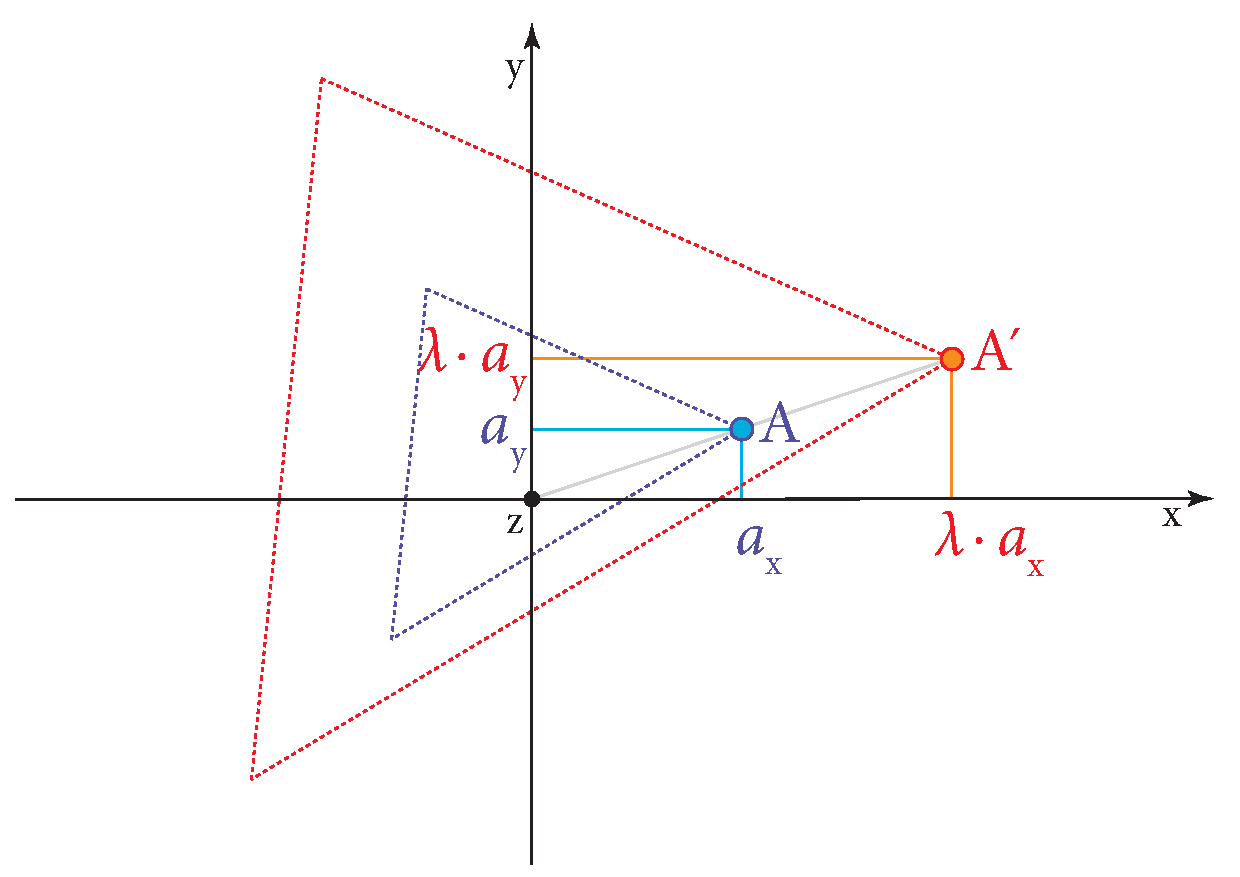
\includegraphics[width=0.49\textwidth]{scaling}
  \vspace{-10pt}
  \caption{Isotrope Skalierung eines Dreiecks um den Faktor $\lambda$.}
\end{wrapfigure}

Die erste und einfachste Transformation, die ich hier vorstellen möchte, ist die Skalierung.

Um ein Objekt zu skalieren, multipliziert man die Koordinaten seiner Eckpunkte jeweils mit einem Skalierungsfaktor $\lambda_i$. Gesucht ist also eine Matrix $S$, für die gilt:
\begin{equation}
 S \cdot
 \begin{pmatrix}
  x \\
  y \\
  z \\
  w
 \end{pmatrix}
 =
 \begin{pmatrix}
  x \cdot \lambda_x \\
  y \cdot \lambda_y \\
  z \cdot \lambda_z \\
  w
 \end{pmatrix}
\end{equation}

Wenn man die Teilgleichung der Multiplikation für eine Koordinate aufstellt (in diesem Fall $x$), erkennt man recht schnell, wie die dazugehörige Zeile der Matrix aussehen muss:
\begin{equation}
\begin{split}
 x \cdot m_{11} + y \cdot m_{12} + z \cdot m_{13} + w \cdot m_{14} = x \cdot \lambda_x \\
 m_{11} = \lambda_x; m_{12} = 0; m_{13} = 0; m_{14} = 0
\end{split}
\end{equation}

Löst man auf die gleiche Weise auch die Teilgleichungen für die anderen Koordinaten, erhält man schließlich folgende Matrix für die \emph{Skalierung um den Koordinatenursprung}:
\begin{equation}
\label{scalingmatrix}
 S{(\lambda_x, \lambda_y, \lambda_z)} =
 \begin{pmatrix}
  \lambda_x & 0 & 0 & 0 \\
  0 & \lambda_y & 0 & 0 \\
  0 & 0 & \lambda_z & 0 \\
  0 & 0 & 0 & 1
 \end{pmatrix}
\end{equation}

Es handelt sich dabei also um eine Diagonalmatrix mit den Skalierungsfaktoren der einzelnen Koordinaten in der Hauptdiagonale (man könnte sie auch als Skalierungsfaktoren der Einheiten der Koordinatenachsen betrachten).

% Quelle: Wikipedia en: Scaling (geometry).
Wenn die Skalierungsfaktoren aller drei Achsen gleich sind, spricht man von einer gleichförmigen oder \emph{isotropen} Skalierung, andernfalls von einer ungleichförmigen oder \emph{antisotropen} Skalierung. Da sich bei einer isotropen Skalierung die Achsen relativ zueinander nicht ändern, sondern auf dreidimensionale Geometrie bezogen nur die Größe des Objektes, wird die isotrope Skalierung zuweilen auch als \emph{Maßstabsänderung} bezeichnet.

Haben alle drei Koeffizienten den Wert $1$, hat die Skalierung keine Auswirkungen -- wie sich leicht überprüfen lässt, ergibt sich aus Gleichung \ref{scalingmatrix} die \emph{Einheitsmatrix}.

Wie man leicht vermuten kann, ist die Skalierung umkehrbar (solange keiner der Faktoren 0 ist). Die inverse Skalierungsmatrix $S^{-1}$ ist dabei die Skalierungsmatrix mit dem Kehrwert der Faktoren:
\begin{equation}
 S^{-1}{(\lambda_x, \lambda_y, \lambda_z)} =
 \begin{pmatrix}
  \frac{1}{\lambda_x} & 0 & 0 & 0 \\
  0 & \frac{1}{\lambda_y} & 0 & 0 \\
  0 & 0 & \frac{1}{\lambda_z} & 0 \\
  0 & 0 & 0 & 1
 \end{pmatrix}
 = S{(\lambda_x^{-1}, \lambda_y^{-1}, \lambda_z^{-1})}
\end{equation}


In manchen Situationen möchte man ein Objekt nicht um den Koordinatenursprung, sondern um einen anderen Punkt im Raum skalieren. In diesem Fall ist die einfachste Lösung, das Objekt zuerst mit einer Translationsmatrix in den Ursprung zu verschieben, die Skalierung durchzuführen und dann das Objekt wieder zurück zu verschieben. Die drei Operationen können in einer Matrix kombiniert werden.

% Matrix 'Skalierung um einen beliebigen Punkt im Raum'?

Die \emph{Spiegelung} kann als Sonderfall der Skalierung betrachtet werden. Dabei sind einer oder mehrere Koeffizienten einen negativen Wert. Eine Spiegelung an der $xy$-Ebene lässt sich beispielsweise als Skalierung mit $\lambda_z = -1$ darstellen.

\section{Translation}
\label{translation}

\begin{wrapfigure}{r}{0.5\textwidth}
  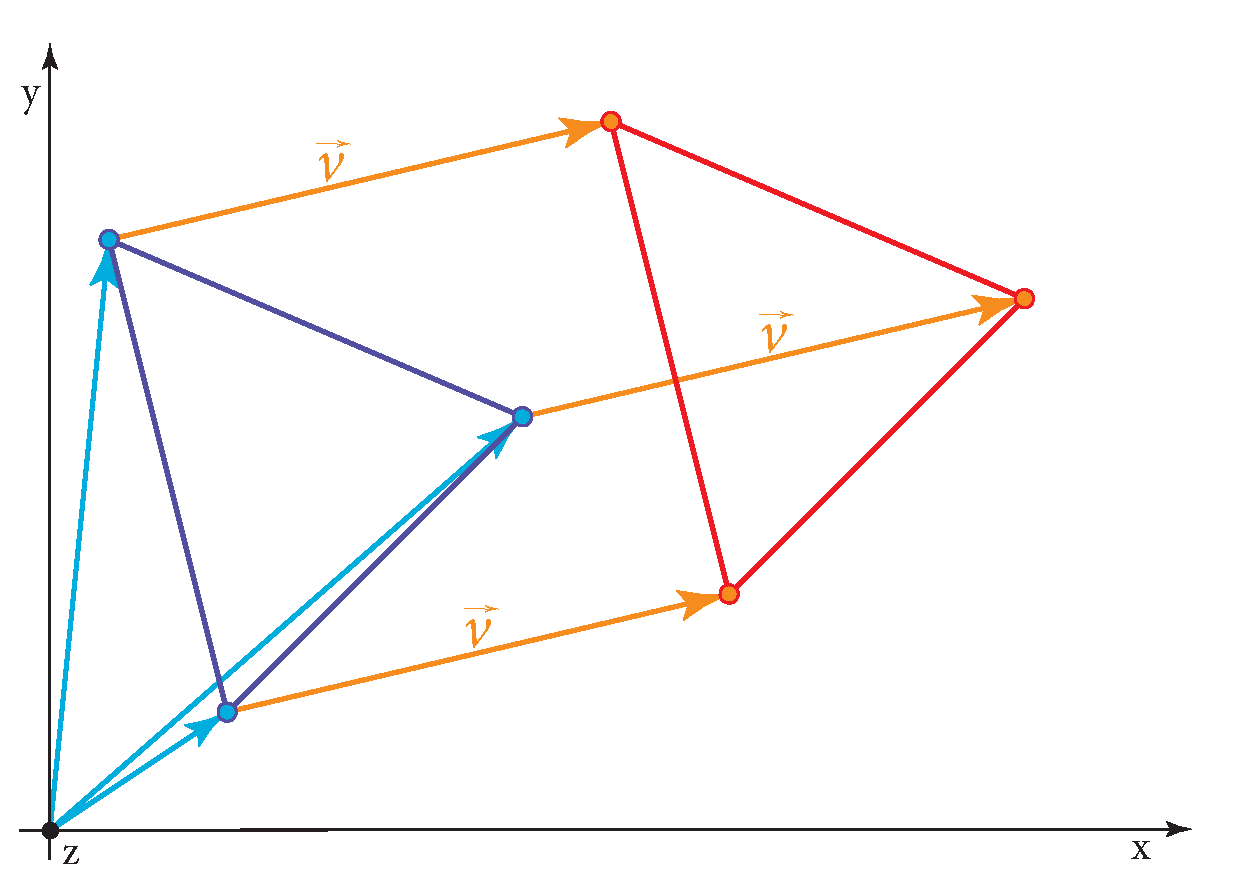
\includegraphics[width=0.49\textwidth]{translation}
  \vspace{-10pt}
  \caption{Translation um $\vec v$.}
\end{wrapfigure}

Die nächste Transformation ist die Translation, also die Verschiebung von Objekten beziehungsweise des Koordinatenursprungs im Raum.

Um alle Eckpunkte eines Objekts um den Vektor $\vec v$ zu verschieben, addiert man die beiden Vektoren einfach nach den Gesetzen der Vektorrechnung komponentenweise. Die gesuchte Translationsmatrix $T$ muss also die folgende Bedingung erfüllen:
\begin{equation}
 T \cdot 
 \begin{pmatrix}
  x \\
  y \\
  z \\
  w
 \end{pmatrix}
 =
 \begin{pmatrix}
  x + v_x \\
  y + v_y \\
  z + v_z \\
  w
 \end{pmatrix}
\end{equation}

Beim Aufstellen der Teilgleichungen (hier exemplarisch für die $y$-Koordinate) wird aber bald ein Problem deutlich:
\begin{equation}
\begin{split}
 x \cdot m_{21} + y \cdot m_{22} + z \cdot & m_{23} + w \cdot m_{24} = y + v_y \\
 m_{21} = 0 \quad m_{23} &= 0 \quad m_{24} = 0 \\
 y \cdot m_{22} & = y + v_y \\
 m_{22} & = \frac{y + v_y}{y} \\
 & = 1 + \frac{v_y}{y}
\end{split}
\end{equation}

Anscheinend gibt es keinen Weg, um die für die Translation nötigen Koeffizienten zu berechnen, ohne die Koordinaten des Vektors zu kennen, der transformiert werden soll. Genau das ist aber Voraussetzung, um die Matrix für mehrere Vektoren verallgemeinern zu können -- die Translation ist offensichtlich keine lineare Transformation!

Der Ausweg aus diesem Dilemma liegt in der Verwendung von homogenen Koordinaten. $w$ hat ja nicht irgendeinen beliebigen Wert, sondern (zumindest vor der Transformation) den Wert $1$. Die dementsprechend geänderten Bedingungen für die Translationsmatrix lauten:
\begin{equation}
 T \cdot 
 \begin{pmatrix}
  x \\
  y \\
  z \\
  1
 \end{pmatrix}
 =
 \begin{pmatrix}
  x + v_x \\
  y + v_y \\
  z + v_z \\
  1
 \end{pmatrix}
\end{equation}

Stellt man nun die Teilgleichung für die $y$-Koordinate auf, erhält man:
\begin{equation}
 x \cdot m_{21} + y \cdot m_{22} + z \cdot m_{23} + 1 \cdot m_{24} = y + v_y
\end{equation}

Diese Bedingung ist einfach erfüllt, indem man
\begin{equation}
 m_{21} = 0; m_{22} = 1; m_{23} = 0; m_{24} = v_y
\end{equation}
setzt.

Auf die gleiche Art kann man auch die anderen Teilgleichungen auflösen. Man erhält als Ergebnis die \emph{Translationsmatrix}
\begin{equation}
 T{(\vec v)} =
 \begin{pmatrix}
  1 & 0 & 0 & v_x \\
  0 & 1 & 0 & v_y \\
  0 & 0 & 1 & v_z \\
  0 & 0 & 0 & 1
 \end{pmatrix}.
\end{equation}

So wie die Skalierung ist auch die Translation einfach umkehrbar. Wenn man die inverse Matrix zu der Translationsmatrix $T{(\vec v)}$ berechnet, kommt man dabei auf
\begin{equation}
 T^{-1}{(\vec v)} =
 \begin{pmatrix}
  1 & 0 & 0 & -v_x \\
  0 & 1 & 0 & -v_y \\
  0 & 0 & 1 & -v_z \\
  0 & 0 & 0 & 1
 \end{pmatrix} = T{(-\vec v)},
\end{equation}
also auf die Verschiebung um einen Vektor gleicher Länge in die entgegengesetzte Richtung.

Wie sich leicht zeigen lässt, kann man, um mehrere Translationen nacheinander auf einen Vektor anzuwenden, einfach die einzelnen Verschiebungsvektoren addieren und so eine gemeinsame Matrix erzeugen:
\begin{equation}
 \label{translationaddition}
 T{(\vec a)} \cdot T{(\vec b)} \cdot \vec p = 
 \begin{pmatrix}
  1 & 0 & 0 & a_x + b_x \\
  0 & 1 & 0 & a_y + b_y \\
  0 & 0 & 1 & a_z + b_z \\
  0 & 0 & 0 & 1
 \end{pmatrix} \cdot \vec p = T{(\vec a + \vec b)} \cdot \vec p
\end{equation}

Dieser Zusammenhang mag trivial erscheinen, aber aus Gleichung \ref{translationaddition} ergibt sich noch eine weitere interessante Eigenheit von Translationsmatrizen: Nachdem die Vektoraddition kommutativ ist, mit der man die Translationen zusammenfassen kann, ist auch die \emph{Multiplikation von Translationsmatrizen kommutativ}.

\section{Rotation}
Die Herleitung der dritten und letzten der hier behandelten Transformationen, der Rotation, ist etwas schwieriger als die vorangegangenen. Am einfachsten ist es, sich zunächst auf die Rotation um eine der Koordinatenachsen zu beschränken, im Folgenden wollen wir zunächst die \emph{Rotation um die z-Achse}, also in der \emph{$xy$-Ebene} betrachten.

\subsection{Rotation um die Koordinatenachsen}

\begin{wrapfigure}{r}{0.5\textwidth}
  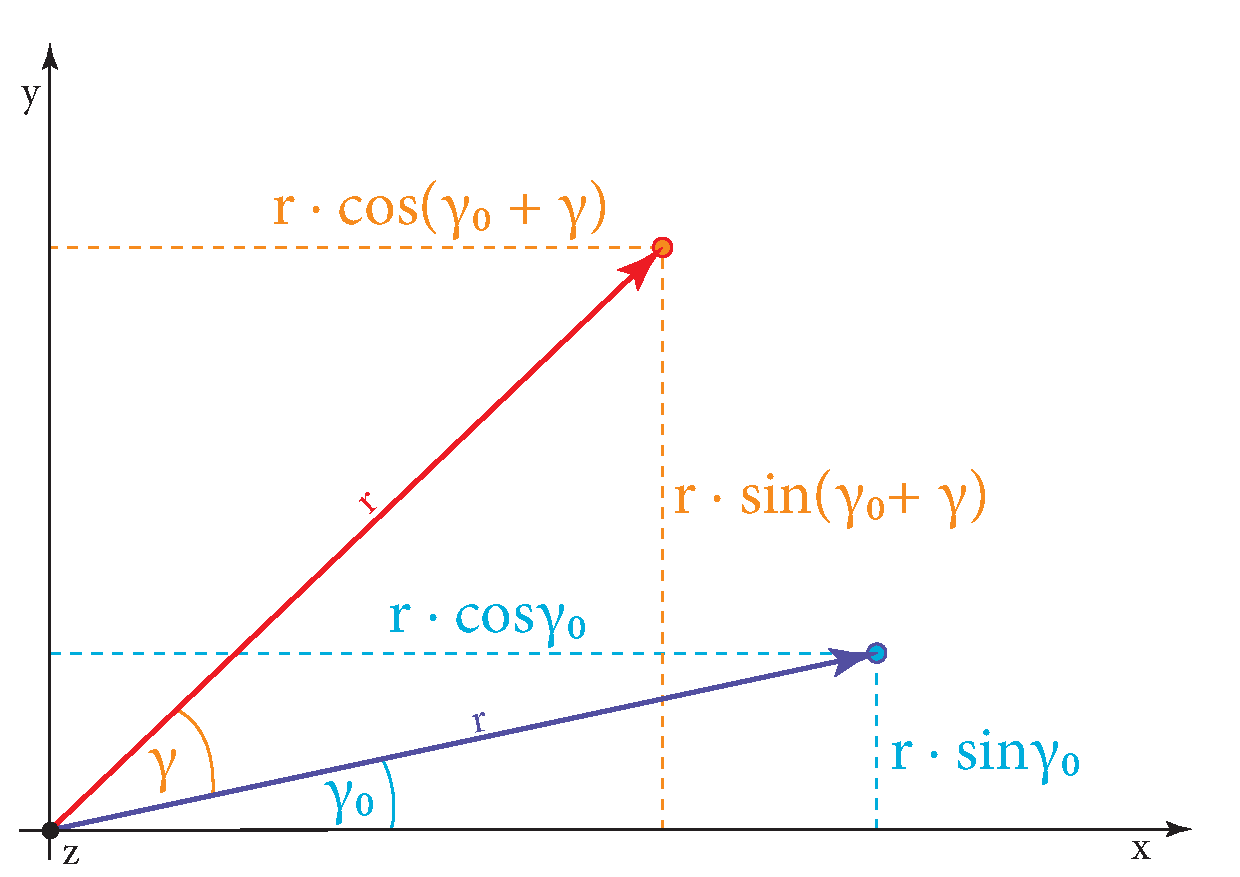
\includegraphics[width=0.49\textwidth]{rotation}
  \vspace{-10pt}
  \caption{Rotation um die $z$-Achse.}
  \label{zrotation}
\end{wrapfigure}

Abbildung \ref{zrotation} zeigt einen Vektor $\vec p = \begin{pmatrix} x & y & z \end{pmatrix}^T$. Nach der Rotation um den Winkel $\gamma$ um die $z$-Achse ergibt sich der Vektor $\vec{p'} = \begin{pmatrix} x' & y' & z' \end{pmatrix}^T$.

Da die Rotation in der $xy$-Ebene stattfindet, ändert sich die $z$-Koordinate des Vektors nicht. Es gilt also
\begin{equation}
 z' = z.
\end{equation}

Für die $x$- und $y$-Koordinaten kann man über die Definition von Sinus und Cosinus ebenfalls direkt aus der Skizze die folgenden Zusammenhänge ableiten:
\begin{align}
  x &= r \cdot \cos{\gamma_0}            &   y &= r \cdot \sin{\gamma_0} \label{rot1} \\
 x' &= r \cdot \cos{(\gamma_0 + \gamma)} &  y' &= r \cdot \sin{(\gamma_0 + \gamma)} \label{rot2}
\end{align}

Unter Zuhilfenahme der trigonometrischen Additionstheoreme erhält man für $x'$ und $y'$ aus \ref{rot2} nach Ausmultiplizieren:
\begin{align}
 \label{rot3}
 x' &= r \cdot \cos \gamma_0 \cos \gamma - r \cdot \sin \gamma_0 \sin \gamma &  y' &= r \cdot \sin \gamma_0 \cos \gamma + r \cdot \cos \gamma_0 \sin \gamma
\end{align}

Die Gleichungen \ref{rot1} ergeben umgeformt:
\begin{align}
 \label{rot4}
 \cos \gamma_0 &= \frac{x}{r} & \sin \gamma_0 &= \frac{y}{r}
\end{align}

Setzt man \ref{rot4} in \ref{rot3} ein, ergibt sich schließlich:
\begin{align}
 x' &= x \cdot \cos \gamma - y \sin \gamma &  y' &= y \cos \gamma + x \sin \gamma
\end{align}

Die gesuchte Rotationsmatrix $R_{z}$ muss also die folgende Bedingung erfüllen:
\begin{equation}
 R_{z} \cdot
 \begin{pmatrix}
  x \\
  y \\
  z \\
  w
 \end{pmatrix}
 = 
 \begin{pmatrix}
  x \cdot \cos \gamma - y \sin \gamma \\
  x \sin \gamma + y \cos \gamma \\
  z \\
  w
 \end{pmatrix}
\end{equation}

Nun ist es ein leichtes, wie für die anderen Transformationen auch die passende Rotationsmatrix für die \emph{Rotation um die $z$-Achse} herzuleiten:
\begin{equation}
 R_z{(\gamma)}
 = 
 \begin{pmatrix}
  \cos \gamma & -\sin \gamma & 0 & 0 \\
  \sin \gamma &  \cos \gamma & 0 & 0 \\
  0 & 0 & 1 & 0 \\
  0 & 0 & 0 & 1 \\
 \end{pmatrix}
\end{equation}

Analog lassen sich auch die Matrizen für die Rotation um die anderen beiden Achsen aufstellen. Man erhält als Ergebnis für die \emph{Rotation um die $x$-Achse}
\begin{equation}
 R_x{(\alpha)}
 = 
 \begin{pmatrix}
  1 & 0 & 0 & 0 \\
  0 & \cos \alpha & -\sin \alpha & 0 \\
  0 & \sin \alpha &  \cos \alpha & 0 \\
  0 & 0 & 0 & 1 \\
 \end{pmatrix}
\end{equation}
% Lz: Vorzeichen korrekt !?

und für die \emph{Rotation um die $y$-Achse}
\begin{equation}
 R_y{(\beta)}
 = 
 \begin{pmatrix}
  \cos \beta & 0 & \sin \beta & 0 \\
  0 & 1 & 0 & 0 \\
  -\sin \beta & 0 & \cos \beta & 0 \\
  0 & 0 & 0 & 1 \\
 \end{pmatrix}.
\end{equation}

Jede Rotation lässt sich selbstverständlich durch nochmalige Rotation um den gleichen Betrag in die andere Richtung umkehren. Beim Aufstellen der inversen Matrix
\begin{equation}
 R_z^{-1}{(\gamma)}
 = 
 \begin{pmatrix}
  \cos \gamma & -\sin \gamma & 0 & 0 \\
  \sin \gamma &  \cos \gamma & 0 & 0 \\
  0 & 0 & 1 & 0 \\
  0 & 0 & 0 & 1 \\
 \end{pmatrix}^{-1}
 = 
 \begin{pmatrix}
   \cos \gamma & \sin \gamma & 0 & 0 \\
  -\sin \gamma & \cos \gamma & 0 & 0 \\
  0 & 0 & 1 & 0 \\
  0 & 0 & 0 & 1 \\
 \end{pmatrix}
 = R_z{(-\gamma)}
\end{equation}
fällt einem auf, dass die Inverse der Rotationsmatrix gleich ihrer Transponierten ist. Dies ist auch tatsächlich eine Eigenheit aller Rotationsmatrizen, beziehungsweise aller Transformationen, bei denen eine beliebige Länge erhalten bleibt.
%Beweis von http://mathworld.wolfram.com/RotationMatrix.html

\subsection{Eulersche Winkel}
Die gerade behandelten Rotationsmatrizen sind auf Drehungen um die Koordinatenachsen beschränkt, aber natürlich lassen sich mehrere der Matrizen kombinieren, um jede beliebige Rotation ausdrücken zu können.

Ein beliebtes Verfahren, um Ausrichtungen im Raum anzugeben, sind die sogenannten Eulerschen Winkel. Dabei handelt es sich um drei Rotationswinkel um jeweils eine Achse, durch die jede beliebige Rotation ausgedrückt werden kann. Es gibt mehrere Konventionen, in welcher Reihenfolge die Rotationen auf welche Achsen angewendet werden. Eine der am häufigsten benutzten sind die aus der Luftfahrt bekannten \emph{Roll-Nick-Gier-Winkel}, auch als \emph{Tait–Bryan-Rotation} bezeichnet (engl. \emph{yaw, pitch, roll}). Sie geben die Rotation als Kombination einer Rotation um die $z$-Achse ($\gamma$), gefolgt von einer Rotation um die $y$-Achse ($\beta$) und schließlich einer Rotation um die $x$-Achse ($\alpha$) an.

Mit einem Wertebereich von $-\pi$ bis $\pi$ für $\alpha$ und $\gamma$ und von $-\frac{\pi}{2}$ bis $\frac{\pi}{2}$ für $\beta$ lassen sich alle Ausrichtungen im Raum angeben. Bis auf zwei Ausnahmen (dazu gleich mehr) ist auch jedem Rotationszustand genau ein Satz an Winkeln zugeordnet, die Abbildung ist also bis auf ebendiese Ausnahmen bijektiv.

Um eine Rotationsdarstellung in Eulerschen Winkeln in Matrixform zu überführen, muss man einfach die Rotationsmatrizen für die einzelnen Achsen miteinander multiplizieren:

\begin{equation}
\begin{split}
 &R_{zyx}( \gamma, \beta, \alpha ) = R_x( \alpha ) \cdot R_y( \beta ) \cdot R_z( \gamma ) \\
 &=
 \begin{pmatrix}
  1 & 0 & 0 & 0 \\
  0 & \cos \alpha & -\sin \alpha & 0 \\
  0 & \sin \alpha &  \cos \alpha & 0 \\
  0 & 0 & 0 & 1 \\
 \end{pmatrix} \cdot
 \begin{pmatrix}
  \cos \beta & 0 & \sin \beta & 0 \\
  0 & 1 & 0 & 0 \\
  -\sin \beta & 0 & \cos \beta & 0 \\
  0 & 0 & 0 & 1 \\
 \end{pmatrix} \cdot
 \begin{pmatrix}
  \cos \gamma & -\sin \gamma & 0 & 0 \\
  \sin \gamma &  \cos \gamma & 0 & 0 \\
  0 & 0 & 1 & 0 \\
  0 & 0 & 0 & 1 \\
 \end{pmatrix} \\
 &=
 \begin{pmatrix}
  \cos \beta \cos \gamma & \cos \beta \sin \gamma & - \sin \beta & 0 \\
  \sin \alpha \sin \beta \cos \gamma - \cos \alpha \sin \gamma & \sin \alpha \sin \beta \sin \gamma + \cos \alpha \cos \gamma & \sin \alpha \cos \beta & 0\\
  \cos \alpha \sin \beta \cos \gamma + \sin \alpha \sin \gamma & \cos \alpha \sin \beta \sin \gamma - \sin \alpha \cos \gamma & \cos \alpha \cos \beta & 0\\
  0 & 0 & 0 & 1
 \end{pmatrix}
\end{split}
\end{equation}

Eulersche Winkel sind ein vergleichbar einfaches und intuitives Mittel, um beliebige Rotationen anzugeben, und werden in der 3D-Grafik gerne für statische Angaben von Rotationen verwendet. Im Bezug auf Animationen haben sie jedoch einige Nachteile:

Zum einen ist es schwer, zwischen zwei in Eulerschen Winkeln gegebenen Rotationszuständen so zu interpolieren, dass die Winkelgeschwindigkeit der resultierenden Rotationsbewegung konstant bleibt. Dies ist für manche Anwendungen wünschenswert, etwa Kamerafahrten, damit die Animation flüssig erscheint.

Zum anderen gibt es wie schon erwähnt für die Zuordnung von Eulerschen Winkeln zu Rotationen zwei kritische Punkte, im Falle der $zyx$-Konvention bei $\beta = \pm \frac{\pi}{2}$, also bei einer Rotation von $90^\circ$ um die $y$-Achse. Setzt man $\frac{\pi}{2}$ in die Matrix ein, erhält man
\begin{equation}
\begin{split}
 R_{zyx}{\left(\alpha, \frac{\pi}{2}, \gamma \right)}
 & = 
 \begin{pmatrix}
  0 & 0 & -1 & 0 \\
  \sin \alpha \cos \gamma - \cos \alpha \sin \gamma & \sin \alpha \sin \gamma + \cos \alpha \cos \gamma & 0 & 0 \\
  \cos \alpha \cos \gamma + \sin \alpha \sin \gamma & \cos \alpha \sin \gamma - \sin \alpha \cos \gamma & 0 & 0 \\
  0 & 0 & 0 & 1
 \end{pmatrix} \\
 & = 
 \begin{pmatrix}
  0 & 0 & -1 & 0 \\
  \sin ( \alpha - \gamma ) &  \cos ( \alpha - \gamma ) & 0 & 0 \\
  \cos ( \alpha - \gamma ) & -\sin ( \alpha - \gamma ) & 0 & 0 \\
  0 & 0 & 0 & 1
 \end{pmatrix}
\end{split}
\end{equation}

Die Rotation hängt nun ausschließlich von der Differenz $\alpha - \gamma$ ab -- das System hat einen Freiheitsgrad eingebüßt! Es gibt jetzt unendlich viele Kombinationen von $\alpha$ und $\gamma$, die zu der gleichen Ausrichtung im Raum führen; die Abbildung der Eulerschen Winkel auf die Rotationsmatrizen ist also nicht injektiv.

Dieses Problem tritt auch bei kardanischen Aufhängungen in der Mechanik auf, beispielsweise bei Trägheitsnavigationssystemen\footnote{Ein echtes Problem ist der Gimbal Lock in der Raumfahrt, wo die kardanische Aufhängung tatsächlich Drehungen um alle drei Freiheitsgrade kompensieren muss. (\vgl irgendein NASA-Dokument)}. Es wird daher als \emph{Gimbal Lock} bezeichnet (engl. \emph{gimbal} bezeichnet einen Kardanring, zu Deutsch also etwa Kardanring-Blockade). In der Mechanik hat man oft die Möglichkeit, Situationen, die zu einem Gimbal Lock führen können, rechtzeitig zu erkennen und den Gimbal Lock zu vermeiden, etwa durch Änderung des Flugmanövers. Bei vom Benutzer ausgelösten oder gesteuerten Rotationen in Computerprogrammen ist dies aber kaum möglich, dewegen greift man normalerweise auf andere Verfahren zurück zurück, um Rotationen zu speichern und zu verarbeiten.
% Picture 'Gimbal lock in mechanics'?

\subsection{Herleitung über transformierte Basisvektoren}
\label{rotationbasevectors}
In den vorigen beiden Abschnitten haben wir die Konstruktion einer Rotationsmatrix ausgehend von einem oder mehreren Rotationswinkeln besprochen. In manchen Fällen kennt man aber bereits die \emph{Basisvektoren} des neuen Koordinatensystems (in den Koordinaten des alten Systems) und will eine Matrix aufstellen, um alle anderen Vektoren zu transformieren.

Hat man drei linear unabhängige Vektoren im alten und im neuen (dreidimensionalen) Koordinatensystem gegeben, lässt sich die Transformationsmatrix $T$ für jede lineare Transformation bestimmen, indem man die Vektoren in die Gleichung $\vec{v'} = T \cdot \vec v$ einsetzt und das Gleichungssystem löst. Daraus ergeben sich allerdings neun Gleichungen in neun Variablen -- händisch eine mühsame und für den Computer eine relativ rechenaufwändige Angelegenheit. Kennt man aber die transformierten \emph{kanonischen Basisvektoren}, \textvec{1}{0}{0}, \textvec{0}{1}{0} und \textvec{0}{0}{1}, vereinfachen sich die Gleichungen wesentlich:

\begin{equation}
 T \cdot \begin{pmatrix} 1 \\ 0 \\ 0 \end{pmatrix} = \begin{pmatrix} x_x \\ x_y \\ x_z \end{pmatrix} \qquad 
\begin{aligned}
 1 \cdot t_{11} + 0 \cdot t_{12} + 0 \cdot t_{13} = t_{11} &= x_x \\
 1 \cdot t_{21} + 0 \cdot t_{22} + 0 \cdot t_{23} = t_{21} &= x_y \\
 1 \cdot t_{31} + 0 \cdot t_{32} + 0 \cdot t_{33} = t_{31} &= x_z
\end{aligned}
\end{equation}

\begin{equation}
 T \cdot \begin{pmatrix} 0 \\ 1 \\ 0 \end{pmatrix} = \begin{pmatrix} y_x \\ y_y \\ y_z \end{pmatrix} \qquad
\begin{aligned}
 0 \cdot t_{11} + 1 \cdot t_{12} + 0 \cdot t_{13} = t_{12} &= y_x \\
 0 \cdot t_{21} + 1 \cdot t_{22} + 0 \cdot t_{23} = t_{22} &= y_y \\
 0 \cdot t_{31} + 1 \cdot t_{32} + 0 \cdot t_{33} = t_{32} &= y_z
\end{aligned}
\end{equation}

\begin{equation}
 T \cdot \begin{pmatrix} 0 \\ 0 \\ 1 \end{pmatrix} = \begin{pmatrix} z_x \\ z_y \\ z_z \end{pmatrix} \qquad
\begin{aligned}
 0 \cdot t_{11} + 0 \cdot t_{12} + 1 \cdot t_{13} = t_{13} &= z_x \\
 0 \cdot t_{21} + 0 \cdot t_{22} + 1 \cdot t_{23} = t_{23} &= z_y \\
 0 \cdot t_{31} + 0 \cdot t_{32} + 1 \cdot t_{33} = t_{33} &= z_z
\end{aligned}
\end{equation}

Für die drei neuen Basisvektoren $\vec x$, $\vec y$ und $\vec z$ entsteht also die Matrix
\begin{equation}
 T(\vec x, \vec y, \vec z) =
 \begin{pmatrix}
  x_x & y_x & z_x \\
  x_y & y_y & z_y \\
  x_z & y_z & z_z \\
 \end{pmatrix},
\end{equation}
beziehungsweise für die Verwendung mit homogenen Koordinaten
\begin{equation}
 T(\vec x, \vec y, \vec z) =
 \begin{pmatrix}
  x_x & y_x & z_x & 0 \\
  x_y & y_y & z_y & 0 \\
  x_z & y_z & z_z & 0 \\
  0 & 0 & 0 & 1
 \end{pmatrix}.
\end{equation}

In Worten ausgedrückt, enthält eine Transformationsmatrix also in ihren Spalten die \emph{Bilder der kanonischen Basisvektoren}.

\subsection{Darstellung als Quaternion}
Wie schon bei der Einführung der Quaternionen in Kapitel \ref{quaternionmath} erwähnt, können Quaternionen als Verbindung eines Skalars und eines dreidimensionalen Vektors aufgefasst werden, wobei der Realteil $w$ den Skalar und der Imaginärteil $xi + yj + zk$ den Vektor \textvec{x}{y}{z} darstellt. Sie eigenen sich deshalb gut für die Darstellung einer Rotation um einen bestimmten Winkel um eine beliebige Achse -- der Rotationswinkel entspricht dem Realteil, die Rotationsachse dem Imaginärteil.

Um mit der Hilfe von Quaternionen die Rotation eines Vektors $\vec x$ um den Winkel $2 \varphi$ mit der Achse $\vec n$ durchzuführen, bildet man zunächst die Quaternion $q = \left[ \cos \varphi; \vec n \cdot \sin \varphi \right]$. Das Ergebnis der Rotation lautet dann $q \cdot \hat{x} \cdot \overline{q}$. Der Vektor $\vec x$ wird hier, wie in Kapitel \ref{quaternionmath} besprochen, als reine Quaternion behandelt. Das Ergebnis der Berechnung ist ebenfalls wieder eine reine Quaternion, kann also wieder als dreidimensionaler Vektor aufgefasst werden. So lautet die Rotationsformel (mit $\left| n \right| = 1$) schließlich:
\begin{equation}
 \hat{x}' = \left[ \cos \varphi; \vec n \cdot \sin \varphi \right] \cdot \hat{x} \cdot \left[ \cos \varphi; -\vec n \cdot \sin \varphi \right]
\end{equation}

\begin{wrapfigure}{r}{0.5\textwidth}
  \vspace{-10pt}
  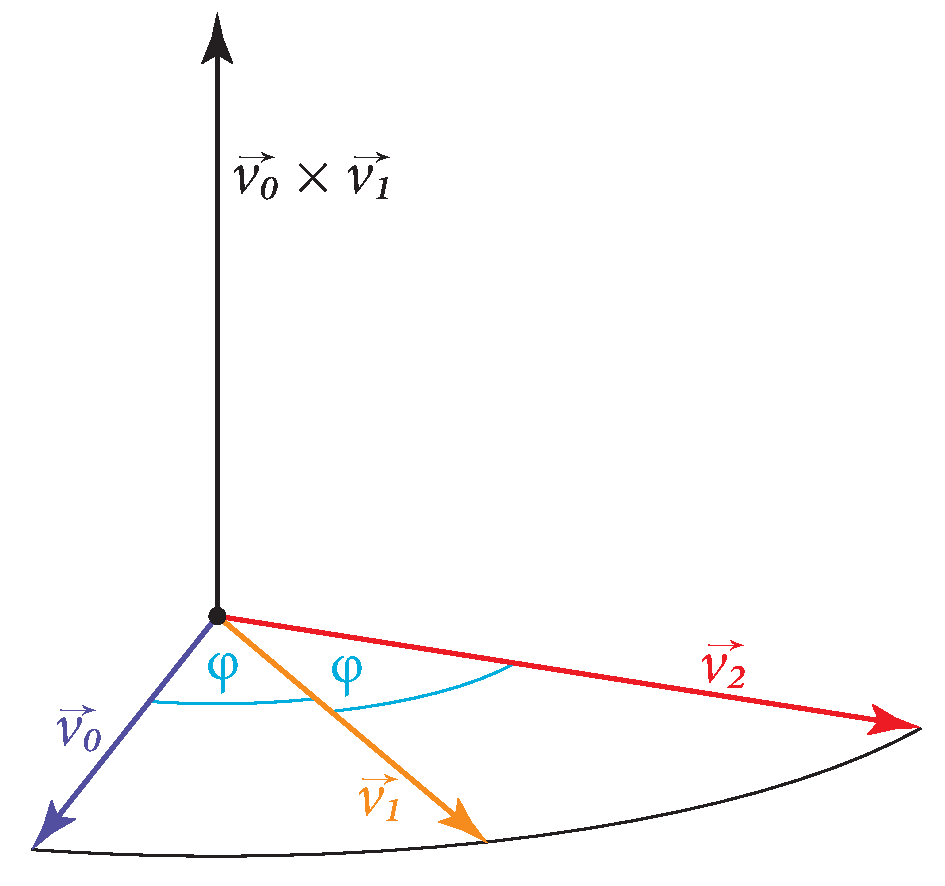
\includegraphics[width=0.49\textwidth]{quatrotation}
  \vspace{-10pt}
  \caption{Rotation um die Achse $\vec{v_0} \times \vec{v_1}$.}
\end{wrapfigure}

Um zu beweisen, dass die oben abgebildete Formel wirklich eine Rotation des Vektors darstellt, betrachten wir zunächst einmal drei Einheitsvektoren $\vec{v_0}$, $\vec{v_1}$ und $\vec{v_2}$ aus dem $\mathbb R^3$ (\vgl \citep{quaternionproof}). Sie sind koplanar und bilden jeweils den Winkel $\varphi$. Es gilt daher:
\begin{align}
 \vec{v_0} \cdot \vec{v_1} = \vec{v_1} \cdot \vec{v_2} = \cos \varphi \label{dotsame} \\
 \vec{v_0} \times\vec{v_1} = \vec{v_1} \times \vec{v_2} \label{crosssame}
\end{align}
$\vec{v_2}$ ensteht also durch eine Rotation von $\vec{v_0}$ um den Winkel $2 \varphi$ mit der Achse $\vec{v_0} \times \vec{v_1}$.

Wir definieren nun die Quaternion $q$ über $\vec{v_0}$ und $\vec{v_1}$:
\begin{equation}
 q = \left[ \left( \vec{v_0} \cdot \vec{v_1} \right); \vec{v_0} \times \vec{v_1} \right]
\end{equation} 

Wir wollen zunächst beweisen:
\begin{equation}
 \label{quaternionclaim}
 q \cdot \hat{v_0} \cdot \overline{q} = p_2
\end{equation} 

Für $q$ gilt
\begin{equation}
 \label{equality1}
 q = \hat{v_1} \cdot \overline{\hat{v_0}},
\end{equation}
weil nach der Multiplikationsvorschrift für Quaternionen (siehe Gleichung \ref{quaternionmultiplicationvector}) gilt:
\begin{equation}
\begin{split}
 \hat{v_1} \cdot \overline{\hat{v_0}} &= \left[ \left( 0 - \vec{v_1} \cdot (-\vec{v_0}) \right); \vec{v_1} \times (-\vec{v_0}) + 0 \cdot (-\vec{v_0}) + 0 \cdot \vec{v_1} \right] \\
 &= \left[ \vec{v_1} \cdot \vec{v_0}; -( \vec{v_1} \times \vec{v_0}) \right] \\
 &= \left[ \vec{v_0} \cdot \vec{v_1}; \vec{v_0} \times \vec{v_1} \right]
\end{split}
\end{equation} 

Dann gilt natürlich auch
\begin{equation}
 \label{equality2}
 q = \hat{v_2} \cdot \overline{\hat{v_1}},
\end{equation} 
weil ja nach Gleichung \ref{dotsame} und \ref{crosssame} die Skalar- und Kreuzprodukte der beiden Vektorenpaare identisch sind.

Wir setzen nun den Zusammenhang aus \ref{equality1} in Gleichung \ref{quaternionclaim} ein und erhalten:
\begin{equation}
\begin{split}
 \label{step1}
 \hat{v_1} \cdot \overline{\hat{v_0}} \cdot \hat{v_0} \cdot \overline{q} &= \hat{v_2} \\
 \hat{v_1} \cdot \left| \hat{v_0} \right| \cdot \overline{q} &= \hat{v_2}
\end{split}
\end{equation}

Nachdem $v_0$ ein Einheitsvektor ist, hat auch $\hat{v_0}$ den Betrag 1, der Ausdruck vereinfacht sich also zu:
\begin{equation}
 \hat{v_1} \cdot \overline{q} = \hat{v_2}
\end{equation}

Nun setzen wir den Zusammenhang aus \ref{equality2} für $\overline{q}$ ein und vereinfachen nach Gleichung \ref{quaternionconjugationmultiplication}:
\begin{equation}
\begin{split}
 \label{step2}
 \hat{v_1} \cdot \overline{\left( \hat{v_2} \cdot \overline{\hat{v_1}} \right)} &= \hat{v_2} \\
 \hat{v_1} \cdot \hat{v_1} \cdot \overline{\hat{v_2}} &= \hat{v_2}
\end{split}
\end{equation}

Nachdem $\hat{v_1}$ eine reine Quaternion und $v_1$ ein Einheitsvektor ist, vereinfacht sich der Ausdruck $\hat{v_1} \cdot \hat{v_1}$:
\begin{equation}
\begin{split}
 \hat{v_1} \cdot \hat{v_1} &= \left[ \left( 0 - \vec{v_1} \cdot \vec{v_1} \right); \vec{v_1} \times \vec{v_1} + 0 \cdot \vec{v_1} + 0 \cdot \vec{v_1} \right] \\
 &= \left[ -\left| \vec{v_1} \right|; \vec 0 \right] \\
 &= -1
\end{split}
\end{equation}

Wir setzen in \ref{step2} ein und erhalten:
\begin{equation}
\begin{split}
 -\overline{\hat{v_2}} &= \hat{v_2} \\
 -\left[ 0; -\vec{v_2} \right] &= \left[ 0; \vec{v_2} \right] \\
 \vec{v_2} &= \vec{v_2}
\end{split}
\end{equation}

Damit wäre der Zusammenhang aus Gleichung \ref{quaternionclaim} bewiesen:
\begin{equation*}
 q \cdot \hat{v_0} \cdot \overline{q} = \hat{v_2}
\end{equation*}

Für $q$ eingesetzt:
\begin{equation*}
 \left[ ( \vec{v_0} \cdot \vec{v_1} ); \vec{v_0} \times \vec{v_1} \right] \cdot \hat{v_0} \cdot \left[ ( \vec{v_0} \cdot \vec{v_1} ); -(\vec{v_0} \times \vec{v_1} ) \right] = \hat{v_2}
\end{equation*} 

Unter Beachtung der Zusammenhänge $\vec a \cdot \vec b = \left| a \right| \cdot \left| b \right| \cdot \cos \varphi$ und $\left| \vec a \times \vec b \right| = \left| a \right| \cdot \left| b \right| \cdot \sin \varphi$ und der Tatsache, dass $\vec{v_0}$ und $\vec{v_1}$ Einheitsvektoren sind, können wir nun einsetzen:
\begin{equation}
 \left[ \cos \varphi; \vec n \cdot \sin \varphi \right] \cdot \hat{v_0} \cdot \left[ \cos \varphi; -\vec n \cdot \sin \varphi \right] = \hat{v_2}
\end{equation}

Nun brauchen wir nur noch beide Seiten mit einem beliebigen Skalar $a$ zu multiplizieren ($\hat{v_0}$ und $\hat{v_2}$ sind ja auf Einheitsquaternionen beschränkt), und es ergibt sich:
\begin{equation}
\begin{split}
 \left[ \cos \varphi; \vec n \cdot \sin \varphi \right] \cdot a \cdot \hat{v_0} \cdot \left[ \cos \varphi; -\vec n \cdot \sin \varphi \right] &= a \cdot \hat{v_2} \\
 \left[ \cos \varphi; \vec n \cdot \sin \varphi \right] \cdot \hat{x} \cdot \left[ \cos \varphi; -\vec n \cdot \sin \varphi \right] &= \hat{x}'
\end{split}
\end{equation}

Wenn die Quaternionen $q_1, q_2, \ldots, q_n$ eine Rotation darstellen, dann lassen sich die Rotationen in eine Quaternion $q$ kombiniern, indem man die Quaterionen -- ähnlich wie bei Transformationsmatrizen -- einfach miteinander multipliziert: $q = q_n \cdot q_{n-2} \cdot \ldots \cdot q_1$. Der zugehörige Beweis ist nahezu trivial: Rotationen zu verketten heißt ja, das Ergebnis der einen Rotation als Ausgangswert für die nächste Transformation zu verwenden. Im Falle von drei Rotationen lautet die Formel also
\begin{equation}
 \hat{x}' = q_3 \cdot ( q_2 \cdot ( q_3 \cdot \hat{x} \cdot \overline{q_1} ) \cdot \overline{q_2} ) \cdot \overline{q_3},
\end{equation}
was wir wegen der Assoziativität der Quaternionenmultiplikation als 
\begin{equation}
 \hat{x}' = ( q_3 \cdot q_2 \cdot q_1 ) \cdot \hat{x} \cdot ( \overline{q_1} \cdot \overline{q_2} \cdot \overline{q_3} )
\end{equation}
schreiben können, was wir gleich zu
\begin{equation}
\begin{split}
 \hat{x}' &= ( q_3 \cdot q_2 \cdot q_1 ) \cdot \hat{x} \cdot \overline{( q_3 \cdot q_2 \cdot q_1 )} \\
 &= q \cdot \hat{x} \cdot \overline{q}
\end{split}
\end{equation} 
vereinfachen können, da sich die Quaternionenmultiplikation ja bezüglich der Konjugation distributiv unter Vertauschung der Reihenfolge verhält (siehe Gleichung \ref{quaternionconjugationmultiplication}).

Quaternionen stellen also wegen ihrer Beziehung zu Rotationswinkel und -achse ein praktisches Mittel dar, um Rotationen anzugeben und mehrere Rotationen können einfach miteinander kombiniert werden (auch im Bezug auf die benötigten Rechenoperationen am Computer). Zusätzlich kann es für manche Computeranwendungen nützlich sein, dass nur vier Werte gespeichert werden müssen, um jede beliebige Rotation darzustellen. Die Repräsentation als Quaternion hat aber auch Nachteile. Zum einen ist die direkte Transformation von Vektoren durch Quaternionen eine relativ rechenaufwändige Angelegenheit, was für den Einsatz in der 3D-Grafik nicht gerade optimal ist. Zum anderen unterstützt die derzeitige Grafikhardware wie in Kapitel \ref{coordinatesystems} beschrieben lediglich Matrizen, um die Vertices zu transformieren. Daher liegt es nahe, einen Weg zu suchen, eine Rotationsquaternion in eine Rotationsmatrix zu konvertieren. (\vgl \citep{rotationissues}, 8-9)

Nachdem ja $\hat{x}'= q \cdot \hat{x} \cdot \overline{q}$ gilt, liegt es nahe, dass man auch nach einer Matrix suchen kann, für die $\vec{x}' = M \cdot \vec{x}$ gilt, die also bei entsprechender Interpretation von reinen Quaternionen als Vektoren die Bedingung $q \cdot \hat{x} \cdot \overline{q} = M \cdot \vec{x}$ erfüllt. Es gibt zahlreiche Wege, die Matrix direkt aus diesem Zusammenhang herzuleiten (\vgl \citep{quaternionrotation}, 56-58; \citep{script:spain}, 93-96), ich möchte aber stattdessen eine andere Möglichkeit zur Herleitung anführen, die leichter nachzuvollziehen ist.

Wie in Abschnitt \ref{rotationbasevectors} besprochen, kann man eine Transformationsmatrix als Aneinanderreihung der transformierten kanonischen Basisvektoren aufstellen. Um eine Matrix aus einem Rotationsquaternion zu erzeugen, muss man also nur die drei Basisvektoren direkt transformieren und die Ergebnisse in die Matrix schreiben.

Dafür multiplizieren wir zunächst einmal die Rotationsformel aus und vereinfachen (\vgl \citep{quaternionrotation}, 52):
\begin{equation}
\begin{split}
 q \cdot \hat{x} \cdot \overline{q} &= \left[ w; \vec n \right] \cdot \left[ 0; \vec x \right] \cdot \left[ w; -\vec n \right] \\
 &= \left[ - \vec n \cdot \vec x; \vec n \times \vec x + w \cdot \vec x \right] \cdot \left[ w; -\vec n \right] \\
 &= \begin{split}[ &- w \cdot ( \vec n \cdot \vec x ) + ( \vec n \times \vec x + w \cdot \vec x ) \cdot \vec n; \\
  &- ( \vec n \times \vec x + w \cdot \vec x ) \times \vec n + w \cdot ( \vec n \times \vec x + w \cdot \vec x ) - \vec n \cdot \vec x \cdot ( - \vec n ) ] \end{split} \\
 &= \begin{split}[ &- w \cdot ( \vec n \cdot \vec x ) + ( \vec n \times \vec x ) \cdot \vec n + w \cdot ( \vec n \cdot \vec x ); \\
  &- ( ( \vec n \times \vec x ) \times \vec n ) - w \cdot ( \vec x \times \vec n ) + w \cdot ( \vec n \times \vec x ) + w^2 \cdot \vec x + ( \vec n \cdot \vec x ) \cdot \vec n ] \end{split} \\
 &= \left[ 0; \vec n \times ( \vec n \times \vec x ) + 2 \cdot w \cdot ( \vec n \times \vec x ) + w^2 \cdot \vec x + ( \vec n \cdot \vec x ) \cdot \vec n \right] \\
 &= \left[ 0; 2 \cdot ( \vec n \cdot \vec x ) \cdot \vec n + 2 \cdot w \cdot ( \vec n \times \vec x ) + ( w^2 - \vec n \cdot \vec n ) \cdot \vec x \right]
\end{split}
\end{equation}

Mithilfe dieser Formel transformieren wir nun die drei Basisvektoren $\vec x$, $\vec y$ und $\vec z$. Für die Komponenten von $\vec x$ erhalten wir:
\begin{equation}
\begin{split}
 x_x' &= 2 \cdot ( x + 0 + 0 ) \cdot x + 2 \cdot w \cdot ( y \cdot 0 - z \cdot 0 ) + ( w^2 - x^2 - y^2 - z^2 ) \cdot 1 \\
      &= x^2 + w^2 - y^2 - z^2 \\
      &= ( 1 - y^2 - z^2 - w^2 ) + w^2 - y^2 - z^2 \\
      &= 1 - 2 \cdot ( y^2 + z^2 )
\end{split}
\end{equation}
\begin{equation}
\begin{split}
 x_y' &= 2 \cdot ( x + 0 + 0 ) \cdot y + 2 \cdot w \cdot ( 1 \cdot z - 0 \cdot x ) + ( w^2 - x^2 - y^2 - z^2 ) \cdot 0 \\
      &= 2xy + 2wz \\
      &= 2 \cdot ( xy + wz )
\end{split}
\end{equation}
\begin{equation}
\begin{split}
 x_z' &= 2 \cdot ( x + 0 + 0 ) \cdot z + 2 \cdot w \cdot ( x \cdot 0 - y \cdot 1 ) + ( w^2 - x^2 - y^2 - z^2 ) \cdot 0 \\
      &= 2xz - 2wy \\
      &= 2 \cdot ( xz + wy )
\end{split}
\end{equation}

Analog werden auch die anderen beiden Vektoren transformiert:
\begin{align}
 \vec{y'} =
 \begin{pmatrix}
  2 \cdot ( xy - wz ) \\
  1 - 2 \cdot ( x^2 + z^2 ) \\
  2 \cdot ( yz + wx )
 \end{pmatrix} \\
 \vec{z'} = 
 \begin{pmatrix}
  2 \cdot ( xz + wy ) \\
  2 \cdot ( yz - wx ) \\
  1 - 2 \cdot ( x^2 + y^2 )
 \end{pmatrix}
\end{align}

Durch Nebeneineinanderstellen von $\vec{x'}$, $\vec{y'}$ und $\vec{z'}$ ergibt sich schließlich die \emph{Rotationsmatrix zu einer Rotationsquaternion $q = w + xi + yj + zk$}
\begin{equation}
 R(q) =
 \begin{pmatrix}
  1 - 2 \cdot ( y^2 + z^2 ) & 2 \cdot ( xy - wz ) & 2 \cdot ( xz + wy ) \\
  2 \cdot ( xy + wz ) & 1 - 2 \cdot ( x^2 + z^2 ) & 2 \cdot ( yz - wx ) \\
  2 \cdot ( xz - wy ) & 2 \cdot ( yz + wx ) & 1 - 2 \cdot ( x^2 + y^2 )
 \end{pmatrix},
\end{equation}
beziehungsweise zur Verwendung mit homogenen Koordinaten
\begin{equation}
 R(q) =
 \begin{pmatrix}
  1 - 2 \cdot ( y^2 + z^2 ) & 2 \cdot ( xy - wz ) & 2 \cdot ( xz + wy ) & 0 \\
  2 \cdot ( xy + wz ) & 1 - 2 \cdot ( x^2 + z^2 ) & 2 \cdot ( yz - wx ) & 0 \\
  2 \cdot ( xz - wy ) & 2 \cdot ( yz + wx ) & 1 - 2 \cdot ( x^2 + y^2 ) & 0 \\
  0 & 0 & 0 & 1
 \end{pmatrix}.
\end{equation}

%\subsection{SLERP und andere Interpolationsverfahren}
% Kapitel 'Betrachtungstransformationen'
\chapter{Betrachtungstransformationen}
\label{viewingtransformations}
Im vorigen Kapitel haben wir die verschiedenen Formen von Skalierung, Translation und Rotation behandelt, die für die Plazierung und Ausrichtung der einzelnen Modelle in der Szene, also für das Berechnen der World Matrix, nötig sind. Das Thema dieses Kapitel ist die Transformationen, die für den Übergang vom Weltkoordinatensystem in das Bildschirmkoordinatensystem verwendet werden.

\section{View Matrix}
\label{view}
In der 3D-Programmierung haben sich zwei praktische Arten eingebürgert, um die Ansicht auf die Szene festzulegen: Die Position des Betrachters kombiniert mit seiner Blickrichtung oder einem Punkt, den er anvisiert. Die View Matrix, die aus diesen Parametern berechnet wird, überführt das Weltkoordinatensystem in das Kamerakoordinatensystem, das seinen Ursprung im Auge des virtuellen Betrachters hat. Die $x$-Achse des neuen Systems zeigt dabei nach rechts, die $y$-Achse nach oben, und die $z$-Achse (in einem rechtshändigen System) gegen die Blickrichtung.

Im ersten Fall sind drei Vektoren gegeben: der Positionsvektor $\vec p$, der Richtungsvektor $\vec d$, und der Hochvektor $\vec u$. Die Bedeutung von $\vec p$ und $\vec u$ sollte klar sein, der Hochvektor ist nötig, um festzulegen, welche Richtung für den Betrachter \enquote{oben} ist. Alle Vektoren haben Einheitslänge, $\vec u$ steht senkrecht auf $\vec d$. Der dritte Basisvektor des neuen Koordinatensystems, der Rechtsvektor $\vec r$, lässt sich leicht über das Kreuzprodukt berechnen:
\begin{equation}
 \vec r = \vec d \times \vec u
\end{equation}

Im zweiten Fall ist neben $\vec p$ nur die Position des Ziels, $\vec t$, gegeben. Der Hochvektor muss aus dem Hochvektor $\vec u_w$ des Weltkoordinatensystems (normalerweise \textvec{0}{1}{0}) berechnet werden. In der Regel wird diese Darstellung in die erste Variante konvertiert, um dann daraus die Matrix zu berechnen. Dazu wird zunächst der normierte Richtungsvektor $\vec d$ berechnet, der von der Position der Kamera zum Ziel zeigt:
\begin{equation}
 \vec d = \frac{\vec t - \vec p}{\left| \vec t - \vec p \right|}
\end{equation}
Der Rechtsvektor muss senkrecht auf der zwischen Welt-Hochvektor und Richtungsvektor aufgespannten Ebene stehen, und lässt sich daher über das Kreuzprodukt gewinnen:
\begin{equation}
 \vec r = \frac{\vec d \times \vec u_w}{\left| \vec d \times \vec u_w \right|}
\end{equation} 
Der Hochvektor berechnet sich nun als Kreuzprodukt aus Rechts- und Richtungsvektor
\begin{equation}
 \vec u = \vec r \times \vec d = \frac{\left( \vec d \times \vec u_w \right) \times \vec d}{\left| \left( \vec d \times \vec u_w \right) \times \vec d \right|},
\end{equation} 
was sich unter Zuhilfenahme der Grassmann-Identität\footnote{$\vec a \times ( \vec b \times \vec c ) = \vec b \cdot ( \vec a \cdot \vec c ) - \vec c \cdot ( \vec a \cdot \vec b)$} zu dem schneller zu berechnenden Ausdruck
\begin{equation}
 \vec u = \frac{ \vec{d} \cdot \left( \vec{u_w} \cdot \vec{d} \right) - \vec{u_w} }{\left| \vec{d} \cdot \left( \vec{u_w} \cdot \vec{d} \right) - \vec{u_w} \right|}
\end{equation} 
vereinfachen lässt.

In beiden Fällen geht es nun darum, aus $\vec p$, $\vec d$, $\vec u$ und $\vec r$ die Transformationsmatrix zu bestimmen. Die Transformation in das Kamerakoordinatensystem kann in zwei Schritte aufgeteilt werden: Zuerst wird der Ursprung des Koordinatensystems in den Standpunkt der Kamera verschoben, dann werden die Achsen korrekt ausgerichtet.

Um den Ursprung in $\vec p$ zu verschieben, müssen alle Objekte um $-\vec p$ verschoben werden:
\begin{equation}
 M_{trans} = \begin{pmatrix}
  1 & 0 & 0 & -p_x \\
  0 & 1 & 0 & -p_y \\
  0 & 0 & 1 & -p_z \\
  0 & 0 & 0 & 1
 \end{pmatrix}
\end{equation}

Die Vektoren $-\vec d$, $\vec u$ und $\vec r$ sind ja die Basisvektoren des Kamarakoordinatensystems, die Matrix für den Rotationsteil kann also wie in Kapitel \ref{rotationbasevectors} beschrieben aufgestellt werden:
\begin{equation}
 M_{rot} =
 \begin{pmatrix}
  r_x & u_x & -d_x & 0 \\
  r_y & u_y & -d_y & 0 \\
  r_z & u_z & -d_z & 0 \\
  0 & 0 & 0 & 1
 \end{pmatrix}
\end{equation}

Um die fertige View Matrix zu erhalten, müssen die beiden Matrizen nur noch multipliziert werden:
\begin{equation}
\begin{split}
 M_{view} &= M_{rot} \cdot M_{trans} \\
 &=
 \begin{pmatrix}
  1 & 0 & 0 & -p_x \\
  0 & 1 & 0 & -p_y \\
  0 & 0 & 1 & -p_z \\
  0 & 0 & 0 & 1
 \end{pmatrix} \cdot
 \begin{pmatrix}
  r_x & u_x & -d_x & 0 \\
  r_y & u_y & -d_y & 0 \\
  r_z & u_z & -d_z & 0 \\
  0 & 0 & 0 & 1
 \end{pmatrix} \\
 M_{view} &=
 \begin{pmatrix}
  r_x & u_x & -d_x & -\vec r \cdot \vec p \\
  r_y & u_y & -d_y & -\vec u \cdot \vec p \\
  r_z & u_z & -d_z & \vec d \cdot \vec p \\
  0 & 0 & 0 & 1
 \end{pmatrix}
\end{split}
\end{equation}

\section{Projection Matrix}
\label{projection}
Die Positionen aller Vertices liegen nach der Transformation durch die View Matrix also im lokalen Koordinatensystem der Kamera vor. Um aus den dreidimensionalen Koordinaten im Raum die zweidimensionalen Bildschirmkoodinaten zu erhalten, müssen sie in irgendeiner Form projiziert werden. Für diese Projektion gibt es je nach Anwendungsgebiet viele Möglichkeiten, darunter auch eher exotische wie die Projektion auf einen Zylindermantel oder krummlinige Projektionen, um Linseneffekte zu simulieren. Aber selbst wenn man sich auf den einfachsten Fall, die Projektion auf eine Ebene, beschränkt, gibt es noch immer zahlreiche Unterarten. \vgls{script:spain}{115-117}

Ich werde mich hier auf die bei Weitem am häufigsten verwendete Art beschränken, die \emph{Zentralprojektion}. Hier wird ein Punkt projiziert, indem man die Linie durch den Punkt und ein gemeinsames Projektionszentrum mit der Bildebene schneidet. Geraden bleiben dabei auch in der Abbildung Geraden, im dreidimensionalen Raum parallele Kanten schneiden sich in einem gemeinsamen Fluchtpunkt. Die Zentralprojektion ist der Abbildung durch das menschliche Auge sehr ähnlich und ermöglicht somit natürlich wirkende Bilder. \vglr{wiki:zentralprojektion}

% Drawing 'Zentralprojektion'

Das \emph{Sichtvolumen} der Zentralprojektion wird also grundsätzlich von den Strahlen durch den Augpunkt und die Ecken des Sichtfensters aufgespannt, ist also eine unendliche rechteckige Pyramide mit der Spitze im Augpunkt \textvec{0}{0}{0}. Die Projektion wird normalerweise durch zwei Parameter charakterisiert: den vertikalen Öffnungswinkel des Sichtvolumens, $\varphi$, und das Seitenverhältnis des Sichtfensters (also im Normalfall des Bildschirmes), $\frac{W}{H} = r$. Wir werden hier nur die normalerweise verwendete \emph{symmetrische Zentralprojektion} behandeln, bei der der Augpunkt in das Zentrum des Bildes projiziert wird.

Wie bereits in Kapitel \ref{coordinatesystems} erwähnt, besteht die Aufgabe der Projection Matrix darin, dieses Sichtvolumen in das \emph{kanonische Sichtvolumen} zu überführen, wonach die Geometrie wieder für alle Arten von Projektion gleich behandelt wird. Auch für das kanonische Sichtvolumen gibt es wieder unterschiedliche Konventionen, wir werden hier die DirectX-Variante behandeln, einen Quader zwischen den Punkten \textvec{-1}{-1}{0} und \textvec{1}{1}{1}.

\begin{wrapfigure}{r}{0.5\textwidth}
  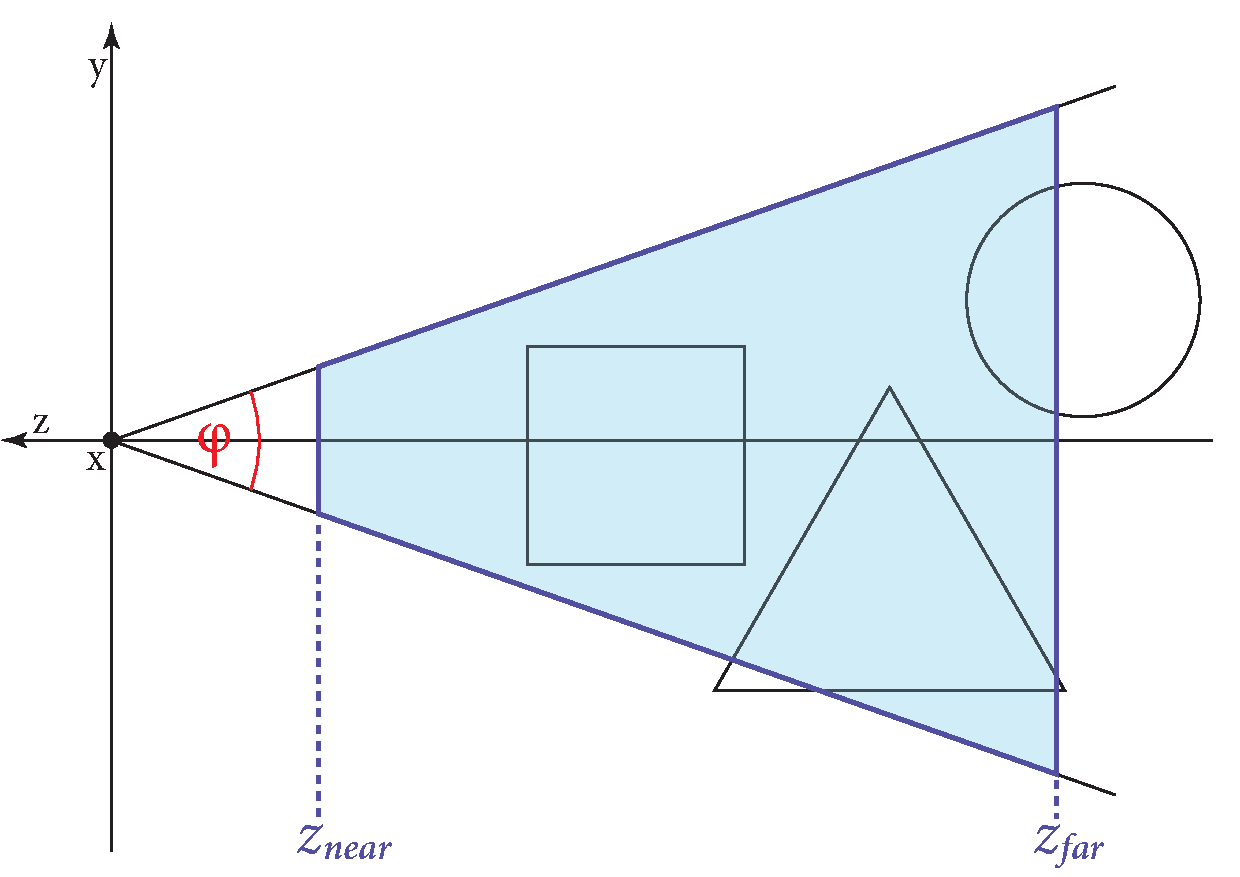
\includegraphics[width=0.49\textwidth]{clippingplanes}
  \caption{Near- und Far Clipping Plane.}
  \label{clippingplanes}
\end{wrapfigure}

Für die Transformation muss das Sichtvolumen aber zuerst begrenzt werden, da sonst verschiedene grundsätzliche und numerische Probleme entstehen werden\footnote{Beispielsweise würden Punkte, die exakt im Augpunkt liegen, ein Problem darstellen.}. Das geschieht mit zwei zur $z$-Achse senkrechten Ebenen, der \emph{Near Clipping Plane} und der \emph{Far Clipping Plane} (von engl. \emph{to clip}, \enquote{abschneiden}). Das entstehende Volumen ist ein Pyramidenstumpf, in der 3D-Grafik meist mit dem englischen Begriff \emph{Frustum} bezeichnet.

Besonders wichtig ist die Begrenzung des Sichtvolumens für die auf die Projektion folgende Sichtbarkeitsbestimmung, da hier wie auch sonst in Computerprogrammen mit einer beschränkten Genaugkeit gerechnet wird. Ist der Abstand von Near und Far Clipping Plane zu groß, macht sich die begrenzte Genauigkeit bemerkbar und es kommt zu einem als \emph{Z-Fighting} bekannten Phänomen, bei dem auf nicht-deterministische Weise abwechselnd verschiedene Pixel von Polygonen in einer ähnlichen Tiefe im Vordergrund gezeichnet werden.

Zur Herleitung der Projection Matrix für die Zentralprojektion transformieren wir das Sichtvolumen zunächst einmal so, dass der horizontale und der vertikale Öffnungswinkel $90^\circ$ betragen ($\varphi = 1$ und $r = 1$). Dazu ist eine Skalierung entlang der $x$- und der $y$-Achse nötig: Wie sich aus Abbildung \ref{clippingplanes} und \ref{rightangledvolume} leicht erkennen lässt, wächst die $y$-Koordinate der oberen und unteren Begrenzung des Frustums bei steigender $z$-Koordinate mit dem Faktor $\pm \tan\frac{\varphi}{2}$, im transformierten Frustum aber mit dem Faktor $\pm 1$. Die $x$-Koordinate der linken und der rechten Grenze verhalten sich bis auf den Faktor für das Seitenverhältnis genauso. Das Sichtvolumen muss also um den Faktor $1 : (\tan\frac{\varphi}{2})$ in $y$-Richtung und $1 : (\tan\frac{\varphi}{2} \cdot r)$ in $x$-Richtung skaliert werden.

\begin{wrapfigure}{r}{0.35\textwidth}
  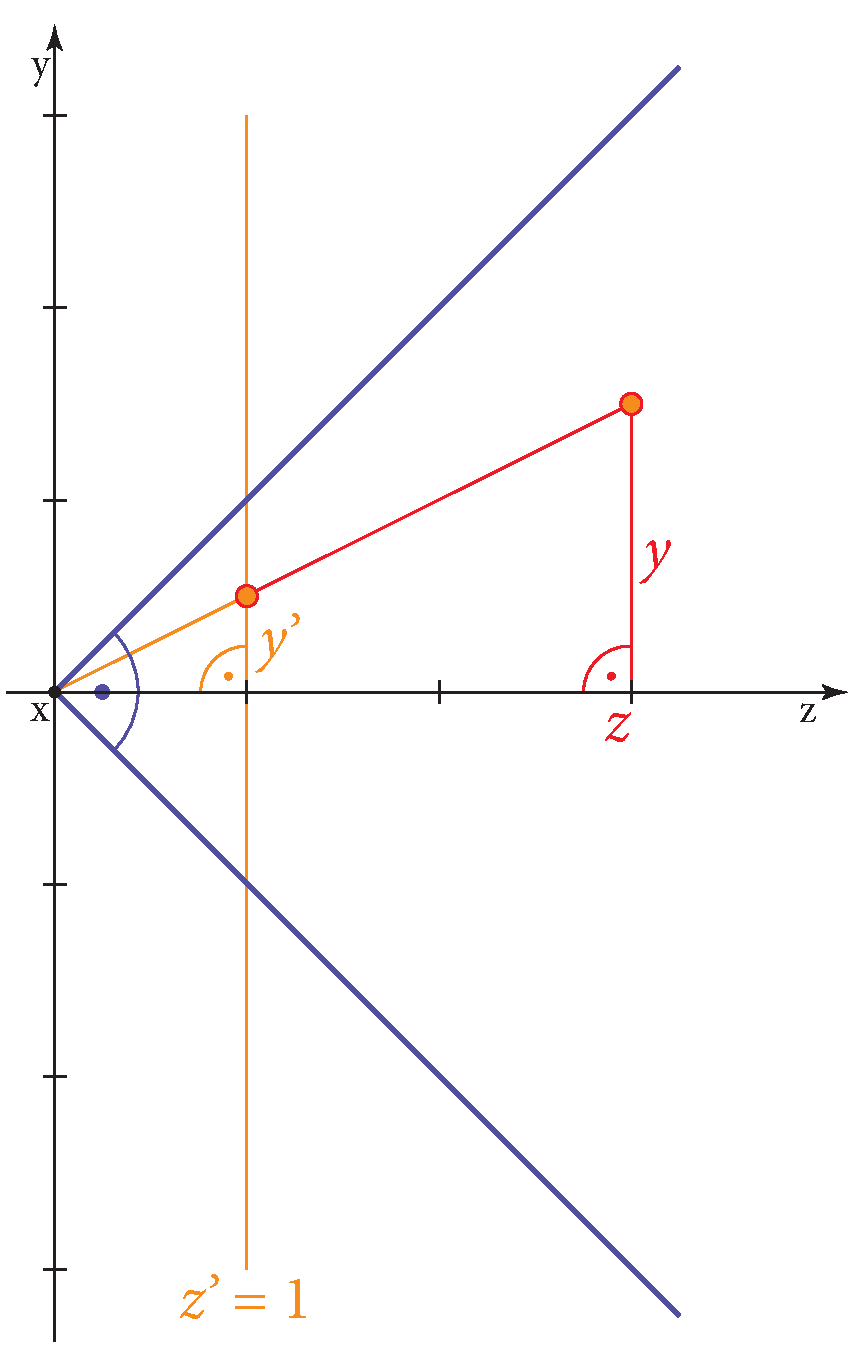
\includegraphics[width=0.34\textwidth]{rightangledvolume}
  \caption{Rechtwinkliges Sichtvolumen mit Projektion auf die Ebene $z=1$.}
  \label{rightangledvolume}
\end{wrapfigure}

Daneben spiegeln wir das Koordinatensystem an der $xy$-Ebene, um ein intuitiveres Arbeiten zu ermöglichen -- mit steigendem Abstand von der Kamera wächst nun auch die $z$-Koordinate. Für diesen ersten Schritt ergibt sich also die Matrix
\begin{equation}
 P_1 = \begin{pmatrix}
  \frac{1}{\tan\frac{\varphi}{2} \cdot r} & 0 & 0 & 0 \\
  0 & \frac{1}{\tan\frac{\varphi}{2}} & 0 & 0 \\
  0 & 0 & -1 & 0 \\
  0 & 0 & 0 & 1
 \end{pmatrix}.
\end{equation}

Danach werden die Punkte auf die Ebene $z=1$ projiziert. Wie aus Abbildung \ref{rightangledvolume} ersichtlich (ähnliche Dreiecke), gilt der Zusammenhang
\begin{equation}
 \frac{x'}{1} = \frac{x}{z}
\end{equation}
und analog für die $y$-Koordinate
\begin{equation}
 \frac{y'}{1} = \frac{y}{z}.
\end{equation}
Um die Projektion durchzuführen, müssen die $x$- und die $y$-Koordinate also durch die $z$-Koordinate dividiert werden. Um dies in eine Matrix zu verpacken, machen wir uns die homogenen Koordinaten zu Nutze, genauer die Konvention, dass der Vektor nachher durch Division durch $w$ wieder auf $w=1$ gebracht wird. Die Matrix braucht also einfach nur $w' = z$ zu setzen
\begin{equation}
 \begin{pmatrix}
  1 & 0 & 0 & 0 \\
  0 & 1 & 0 & 0 \\
  0 & 0 & 1 & 0 \\
  0 & 0 & 1 & 0
 \end{pmatrix}.
\end{equation}
Nach der Transformation mit dieser Matrix hat ein Vektor die Koordinaten \textvech{x}{y}{z}{z}, nach der homogenen Division also \textvec{\frac{x}{z}}{\frac{y}{z}}{1}.

Für die Projektion reicht diese Transformation an sich, und wie man leicht nachprüfen kann, befinden sich die $x$- und $y$-Koordinaten alle Punkte im Sichtvolumen jetzt zwischen $-1$ und $1$, wie es für das kanonische Sichtvolumen erforderlich ist. Allerdings ist durch die Projektion auch $z'$ für alle Punkte $1$, ist also unabhängig von $z$. Um später beim Zeichnen der Dreiecke die Sichtbarkeit korrekt bestimmen zu können, muss $z'$ aber mit wachsender Tiefe monoton steigen, die $z$-Reihenfolge der Punkte muss also erhalten bleiben. Um diese Bedingung zu erfüllen, werden zwei zusätzliche Parameter, $a$ und $b$, eingeführt:
\begin{equation}
 \begin{pmatrix}
  1 & 0 & 0 & 0 \\
  0 & 1 & 0 & 0 \\
  0 & 0 & a & b \\
  0 & 0 & 1 & 0
 \end{pmatrix}.
\end{equation}

Nach der Transformation und der homogenen Division ergibt sich mit dieser Matrix
\begin{equation}
 z' = \frac{a \cdot z + b}{z}.
\end{equation}

Nun müssen nur noch passende Werte für $a$ und $b$ gefunden werden. Aus der Definition des kanonischen Sichtvolumens folgen ja die Bedingungen, dass ein Punkt auf der Near Clipping Plane auf $z'=0$, und ein Punkt auf der Far Clipping Plane auf $z'=1$ abgebildet wird. Aus diesen Bedingungen ergibt sich also ein lineares Gleichungssystem mit zwei Variablen
\begin{equation}
\begin{split}
 0 = \frac{a \cdot z_{near} + b}{z_{near}} \\
 1 = \frac{a \cdot z_{far} + b}{z_{far}},
\end{split}
\end{equation}
welches sich einfach zu
\begin{equation}
\begin{split}
 a = \frac{z_{far}}{z_{far}-z_{near}} \\
 b = -z_{near} \cdot a = -\frac{z_{far} \cdot z_{near}}{z_{far}-z_{near}},
\end{split} 
\end{equation}
auflösen lässt. \vglr{perspectiveprojectionmatrix}

Für die Projektion des rechtwinkligen Sichtvolumens ergibt sich also die Matrix
\begin{equation}
 P_2 = \begin{pmatrix}
  1 & 0 & 0 & 0 \\
  0 & 1 & 0 & 0 \\
  0 & 0 & \frac{z_{far}}{z_{far}-z_{near}} & -\frac{z_{far} \cdot z_{near}}{z_{far}-z_{near}} \\
  0 & 0 & 1 & 0
 \end{pmatrix}.
\end{equation}

Kombiniert man die beiden Matrizen durch Multiplikation, erhält man die \emph{Projection Matrix für die Zentralprojektion}:
\begin{equation}
 M_{proj} = P_2 \cdot P_1 = 
 \begin{pmatrix}
  \frac{1}{\tan\frac{\varphi}{2} \cdot r} & 0 & 0 & 0 \\
  0 & \frac{1}{\tan\frac{\varphi}{2}} & 0 & 0 \\
  0 & 0 & -\frac{z_{far}}{z_{far}-z_{near}} & \frac{z_{far} \cdot z_{near}}{z_{far}-z_{near}} \\
  0 & 0 & 1 & 1
 \end{pmatrix}
\end{equation} 

Nach der Transformation mit dieser Matrix befinden sich alle sichtbaren Dreiecke im kanonischen Sichtvolumen. Auf die Projektion folgt nun, wie in Kapitel \ref{rendering} beschrieben, das \emph{Clipping}. Dabei werden alle Dreiecke, die nicht vollständig innerhalb des kanonischen Sichtvolumens liegen, abgeschnitten beziehungsweise überhaupt verworfen, wenn sie ganz außerhalb liegen.

Viewport-Koordinaten

\appendix
% Anhang 'Beispielprogramm'
\chapter{Beispielprogramm}
\label{beispielprogramm}

Wie schon in der Einleitung erwähnt, habe ich mich während der letzten Monate nicht nur mit dem theoretischen Teil der 3D-Grafik auseinandergesetzt, sondern auch ein praktisches Projekt umgesetzt: einen kleinen Software-Renderer mit dem äußerst kreativen Namen \enquote{d4}, geschrieben in der Programmiersprache~D.

Bei einem Software Renderer handelt es sich um ein Programm, dass die 3D-Pipeline in Software implementiert, die Berechnungen also ausschließlich auf dem Hauptprozessor des Computers ausführt. Diese Vorgehensweise ist eigentlich seit Mitte der 90er-Jahre überholt \vglr{wiki:grafikkarte}, da mit der in praktisch allen PCs vorhandenen Grafikkarte ein hoch spezialisiertes und viel effizienteres Mittel zu Verfügung steht, um die Berechnungen durchzuführen. Beim Programmieren eines Software Renderers ist man aber gezwungen, sich mit vielen interessanten Details auseinanderzusetzen, über die man sich normalerweise dank leistungsfähriger Hardware und abstrahierender Programmierschnittstellen nicht weiter den Kopf zerbrechen muss.

Das Projekt ist auf der beiliegenden CD im Verzeichnis \path{d4} zu finden. Im Unterverzeichnis \path{src} befindet sich der Quellcode des Programmes. Die Dateien im Paket \path{assimp} lediglich eine 1:1-Übertragung der C-Schnittstelle der Assimp-Bibliothek, im Gegensatz zu den restlichen Programmteilen also nicht als meine eigene Arbeit zu betrachten. Die Dokumentation des Quellcodes sollte ausreichend genau sein, um Ihnen zu ermöglichen, darin zu stöbern. Ebenfalls nur für Programmierer interessant dürfte das Unterverzeichnis \path{build} sein. Es enhält die Konfigurationsdatei für das Programm \emph{dsss}\footnote{\url{http://www.dsource.org/projects/dsss}}, mit dessen Hilfe das Projekt neu aus den Quellen erstellt werden kann.

Das Unterverzeichnis \path{bin} enthält die ausführbaren Dateien für Windows (\path{d4.exe}) und Linux (\path{d4}). Zum Ausführen des Programmes sind einige externe Bibliotheken erforderlich, nämlich die Multimedia-Bibliothek \emph{SDL}\footnote{\url{http://www.libsdl.org/}}, die Bibliothek \emph{Assimp}\footnote{\url{http://assimp.sourceforge.net/}} zum Einlesen der Modelldateien und die Bibliothek \emph{DevIL}\footnote{\url{http://openil.sourceforge.net/}} zum Laden der Texturen. Die aktuellen Versionen der erforderlichen DLL-Dateien für die 32\,bit-Versionen von Microsoft Windows befinden sich bereits im \path{bin}-Verzeichnis, sodass in den meisten Fällen keine zusätzlichen Schritte nötig sein sollten. Unter Linux müssen die entsprechenden Pakete der Distribution installiert sein. Für den Fall, dass dies nicht ausreichen sollte, habe ich im Verzeichnis \path{bin/libraries} die Quellpakete beigelegt, aus denen sich die drei Bibliotheken bei Bedarf kompilieren lassen.
% @todo: Benötigte Versionen.

Das Programm erwartet als ersten Parameter den Namen der Modelldatei, die geladen werden soll. Dank der beiden exzellenten Bibliotheken werden jeweils knapp 30 mehr oder weniger verbreitete Modell- und Texturformate unterstüzt, eine genaue Auflistung findet sich auf den Websites der Bibliotheken und in der beiliegenden \path{README}-Datei. Der Parameter kann natürlich angegeben werden, wenn das Programm von der Kommandozeile gestartet wird. Unter Windows dürfte es jedoch leichter sein, einfach eine Verknüpfung zu der \path{.exe}-Datei an geigneter Stelle (beispielsweise auf dem Desktop) anzulegen, und dann einfach eine Modelldatei per \emph{Drag\,\&\,Drop} auf die Verknüpfung \enquote{fallen zu lassen}. Im Verzeichnis \path{bin/models} befinden sich neben einigen einfachen geometrischen Grundkörpern auch zwei Modelle eines Fantasy-Zwerges von einem Künstlers mit dem Pseudonym \emph{Psionic}, die sich einer Textur bedienen.

Das Programm akzeptiert noch zwei optionale Parameter: Mit dem Parameter \argument{fakeColors} wird jeder Eckpunkt in einer eigenen Farbe gezeichnet, wodurch die dem Modell zugrundeliegende Struktur sichtbar gemacht wird. \argument{smoothNormals} weist das Programm an, beim Importieren von Modellen ohne Vertexnormalen Normalvektoren zu generieren, die eine \enquote{glatte} Oberfläche erzeugen (siehe Kapitel \ref{vertexnormals}).

Noch ein paar Worte zur Bedienung: Die Kamera kann mittels der Tasten \key{W}, \key{S}, \key{A} und \key{D} bewegt und mit den Pfeiltasten gedreht werden. Die \key{Shift}- bzw. \key{Umschalt}-Taste beschleunigt dabei die Bewegungen. Die Tasten in der unteren Reihe das Tastatur steuern verschiedene Funktionen des Programms: \key{Y} wechselt zwischen Flat Shading, Gouraud Shading und Gouraud Shading mit Texturen; \key{X} schaltet den Wireframe-Modus ein und aus; \key{C} steuert das Backface-Culling; \key{V} lässt die Welt um den Koordinatenursprung drehen; \key{B} erzeugt einen animierten Farbverlauf im Hintergrund. Ein Druck auf die \key{Esc}-Taste beendet das Programm.

\listoffigures

\bibliographystyle{dinat}
\bibliography{3d-mathematics}

\end{document}
